% From https://github.com/UWIT-IAM/UWThesis
\documentclass[print]{nuthesis}
\usepackage{amssymb, amsthm, amsmath, amsfonts}
\usepackage{wasysym}
\usepackage{mathrsfs}
% \usepackage{hyperref}
\usepackage{graphicx}
\usepackage{lineno}
\usepackage[colorinlistoftodos]{todonotes}
\usepackage{listings}
%\usepackage{breqn}
\usepackage{cancel, enumerate}
\usepackage{rotating, environ}
\usepackage{caption}
\usepackage{subcaption}
\usepackage[inline]{enumitem}
\usepackage{dirtree}

\newtheorem{thm}{Theorem}
\newtheorem{defn}{Definition}
\newtheorem{prop}{Proposition}
\newtheorem{lemma}{Lemma}
\newtheorem{cor}{Corollary}

% Syntax highlighting #22
  \usepackage{color}
  \usepackage{fancyvrb}
  \newcommand{\VerbBar}{|}
  \newcommand{\VERB}{\Verb[commandchars=\\\{\}]}
  \DefineVerbatimEnvironment{Highlighting}{Verbatim}{commandchars=\\\{\}}
  % Add ',fontsize=\small' for more characters per line
  \usepackage{framed}
  \definecolor{shadecolor}{RGB}{248,248,248}
  \newenvironment{Shaded}{\begin{snugshade}}{\end{snugshade}}
  \newcommand{\AlertTok}[1]{\textcolor[rgb]{0.94,0.16,0.16}{#1}}
  \newcommand{\AnnotationTok}[1]{\textcolor[rgb]{0.56,0.35,0.01}{\textbf{\textit{#1}}}}
  \newcommand{\AttributeTok}[1]{\textcolor[rgb]{0.77,0.63,0.00}{#1}}
  \newcommand{\BaseNTok}[1]{\textcolor[rgb]{0.00,0.00,0.81}{#1}}
  \newcommand{\BuiltInTok}[1]{#1}
  \newcommand{\CharTok}[1]{\textcolor[rgb]{0.31,0.60,0.02}{#1}}
  \newcommand{\CommentTok}[1]{\textcolor[rgb]{0.56,0.35,0.01}{\textit{#1}}}
  \newcommand{\CommentVarTok}[1]{\textcolor[rgb]{0.56,0.35,0.01}{\textbf{\textit{#1}}}}
  \newcommand{\ConstantTok}[1]{\textcolor[rgb]{0.00,0.00,0.00}{#1}}
  \newcommand{\ControlFlowTok}[1]{\textcolor[rgb]{0.13,0.29,0.53}{\textbf{#1}}}
  \newcommand{\DataTypeTok}[1]{\textcolor[rgb]{0.13,0.29,0.53}{#1}}
  \newcommand{\DecValTok}[1]{\textcolor[rgb]{0.00,0.00,0.81}{#1}}
  \newcommand{\DocumentationTok}[1]{\textcolor[rgb]{0.56,0.35,0.01}{\textbf{\textit{#1}}}}
  \newcommand{\ErrorTok}[1]{\textcolor[rgb]{0.64,0.00,0.00}{\textbf{#1}}}
  \newcommand{\ExtensionTok}[1]{#1}
  \newcommand{\FloatTok}[1]{\textcolor[rgb]{0.00,0.00,0.81}{#1}}
  \newcommand{\FunctionTok}[1]{\textcolor[rgb]{0.00,0.00,0.00}{#1}}
  \newcommand{\ImportTok}[1]{#1}
  \newcommand{\InformationTok}[1]{\textcolor[rgb]{0.56,0.35,0.01}{\textbf{\textit{#1}}}}
  \newcommand{\KeywordTok}[1]{\textcolor[rgb]{0.13,0.29,0.53}{\textbf{#1}}}
  \newcommand{\NormalTok}[1]{#1}
  \newcommand{\OperatorTok}[1]{\textcolor[rgb]{0.81,0.36,0.00}{\textbf{#1}}}
  \newcommand{\OtherTok}[1]{\textcolor[rgb]{0.56,0.35,0.01}{#1}}
  \newcommand{\PreprocessorTok}[1]{\textcolor[rgb]{0.56,0.35,0.01}{\textit{#1}}}
  \newcommand{\RegionMarkerTok}[1]{#1}
  \newcommand{\SpecialCharTok}[1]{\textcolor[rgb]{0.00,0.00,0.00}{#1}}
  \newcommand{\SpecialStringTok}[1]{\textcolor[rgb]{0.31,0.60,0.02}{#1}}
  \newcommand{\StringTok}[1]{\textcolor[rgb]{0.31,0.60,0.02}{#1}}
  \newcommand{\VariableTok}[1]{\textcolor[rgb]{0.00,0.00,0.00}{#1}}
  \newcommand{\VerbatimStringTok}[1]{\textcolor[rgb]{0.31,0.60,0.02}{#1}}
  \newcommand{\WarningTok}[1]{\textcolor[rgb]{0.56,0.35,0.01}{\textbf{\textit{#1}}}}

%% https://github.com/rstudio/rmarkdown/issues/1649
\newlength{\cslhangindent}
\setlength{\cslhangindent}{1.5em}
\newenvironment{CSLReferences}[2]%
{\setlength{\parindent}{0pt}%
\everypar{\setlength{\hangindent}{\cslhangindent}}\ignorespaces}%
{\par}

% fix for pandoc 1.14
\providecommand{\tightlist}{%
  \setlength{\itemsep}{0pt}\setlength{\parskip}{0pt}}

%% something about tables, from https://github.com/ismayc/thesisdown/issues/122
\usepackage{calc}

%% for copyright symbol
\usepackage{textcomp}

%% to allow to rotate pages to landscape
\usepackage{lscape}
%% to adjust table column width
\usepackage{tabularx}

% suppress bottom page numbers on first page of each chapter
% because they overlap with text
\usepackage{etoolbox}
\patchcmd{\chapter}{plain}{empty}{}{}

%% for more attractive tables
\usepackage{booktabs}
\usepackage{longtable}


\usepackage{graphicx}


% Double spacing, if you want it.
\def\dsp{\def\baselinestretch{2.0}\large\normalsize}
% \dsp

% If the Grad. Division insists that the first paragraph of a section
% be indented (like the others), then include this line:
\usepackage{indentfirst}

%%%%%%%%%%%%%%%%%%
% If you want to use "sections" to partition your thesis
% un-comment the following:
%
% \counterwithout{section}{chapter}
% \setsecnumdepth{subsubsection}
% \def\sectionmark#1{\markboth{#1}{#1}}
% \def\subsectionmark#1{\markboth{#1}{#1}}
% \renewcommand{\thesection}{\arabic{section}}
% \renewcommand{\thesubsection}{\thesection.\arabic{subsection}}
% \makeatletter
% \let\l@subsection\l@section
% \let\l@section\l@chapter
% \makeatother

\renewcommand{\thetable}{\arabic{table}}
\renewcommand{\thefigure}{\arabic{figure}}

%%%%%%%%%%%%%%%%%%


%% Stuff from https://github.com/suchow/Dissertate

% The following line would print the thesis in a postscript font

% \usepackage{natbib}
% \def\bibpreamble{\protect\addcontentsline{toc}{chapter}{Bibliography}}

\setcounter{tocdepth}{1} % Print the chapter and sections to the toc
% controls depth of table of contents (toc): 0 = chapter, 1 = section, 2 = subsection

\usepackage{natbib}


% commands and environments needed by pandoc snippets
% extracted from the output of `pandoc -s`
%% Make R markdown code chunks work
\usepackage{array}
\usepackage{amssymb,amsmath}
\usepackage{ifxetex,ifluatex}
\ifxetex
  \usepackage{fontspec,xltxtra,xunicode}
  \defaultfontfeatures{Mapping=tex-text,Scale=MatchLowercase}
\else
  \ifluatex
    \usepackage{fontspec}
    \defaultfontfeatures{Mapping=tex-text,Scale=MatchLowercase}
  \else
    \usepackage[utf8]{inputenc}
  \fi
\fi
\usepackage{color}
\usepackage{fancyvrb}


\ifxetex
  \usepackage[setpagesize=false, % page size defined by xetex
              unicode=false, % unicode breaks when used with xetex
              xetex,
              colorlinks=true,
              linkcolor=blue]{hyperref}
\else
  \usepackage[unicode=true,
              colorlinks=true,
              linkcolor=blue]{hyperref}
\fi
\hypersetup{breaklinks=true, pdfborder={0 0 0}}
\setlength{\parindent}{20pt}
\setlength{\parskip}{6pt plus 2pt minus 1pt}
\setlength{\emergencystretch}{3em}  % prevent overfull lines
\setcounter{secnumdepth}{2} %% controls section numbering, e.g. 1 or 1.2, or 1.2.3



%  ----  Text Colors  ------------------------------------------
%
% Assign colors to writers for review
%
\newcommand{\db}[1]{{\textcolor{blue}{#1}}}
\newcommand{\svp}[1]{{\textcolor{RedOrange}{#1}}}
\newcommand{\cochaircol}[1]{{\textcolor{Green}{#1}}}
%


%  --- Code chunk font size -----------------------------------------------
% https://stackoverflow.com/questions/38323331/code-chunk-font-size-in-beamer-with-knitr-and-latexhttps://stackoverflow.com/questions/38323331/code-chunk-font-size-in-beamer-with-knitr-and-latex

%% change fontsize of R code
\let\oldShaded\Shaded
\let\endoldShaded\endShaded
\renewenvironment{Shaded}{\footnotesize\oldShaded}{\endoldShaded}

%% change fontsize of output
\let\oldverbatim\verbatim
\let\endoldverbatim\endverbatim
\renewenvironment{verbatim}{\footnotesize\oldverbatim}{\endoldverbatim}


\begin{document}
% \linenumbers{}
%% Start formatting the first few special pages
%% frontmatter is needed to set the page numbering correctly
\frontmatter
%% from thesisdown
% To pass between YAML and LaTeX the dollar signs are added by CII
\title{DATA SCIENCE, DASHBOARDS, AND THE WAY IT WORKS WITH STATISTICS}
\author{Denise Renee Bradford}
\adviser{Susan R. VanderPlas, Ph.D}
% \adviserAbstract{}
\major{Statistics}
\degreemonth{Month}
\degreeyear{Year}
% \copyrightpage
%%
%% For most people the defaults will be correct, so they are commented
%% out. To manually set these, just uncomment and make the needed
%% changes.
%% \college{Your college}
%% \city{Your City}
%%
%% For most people the following can be changed with a class
%% option. To manually set these, just uncomment the following and
%% make the needed changes.
%% \doctype{Thesis or Dissertation}
%% \degree{Your degree}
%% \degreeabbreviation{Your degree abbr.}
%%
%% Now that we know everything we need, we can generate the title page
%% itself.
%%
\maketitle


\begin{abstract}
    Here is my abstract. \emph{(350 word limit)}
\end{abstract}

%% Optional
\begin{copyrightpage}
\end{copyrightpage}

%% Optional
\begin{dedication}
Dedicated to\ldots{}
\end{dedication}

%%%%%%%%%%%%%%%%%%%
% Acknowledgments
%%%%%%%%%%%%%%%%%%%
\begin{acknowledgments}
Thank you to all my people!
\end{acknowledgments}
%%%%%%%%%%%%%%%%%%%

%%%%%%%%%%%%%%%%%%%
% Grant Information
%%%%%%%%%%%%%%%%%%%
% \begin{grantinfo}
%     % Add any grant info here
% \end{grantinfo}

%%%%%%%%%%%%%%%%%%%
% ToC
%%%%%%%%%%%%%%%%%%%
\tableofcontents

%%%%%%%%%%%%%%%%%%%
% List of Figures
%%%%%%%%%%%%%%%%%%%
\listoffigures
\listoftables

%%%%%%%%%%%%%%%%%%%
% Start of the document
%%%%%%%%%%%%%%%%%%%
\mainmatter


\hypertarget{literature-review}{%
\chapter{Literature Review}\label{literature-review}}

\hypertarget{introduction}{%
\section{Introduction}\label{introduction}}

\begin{center}
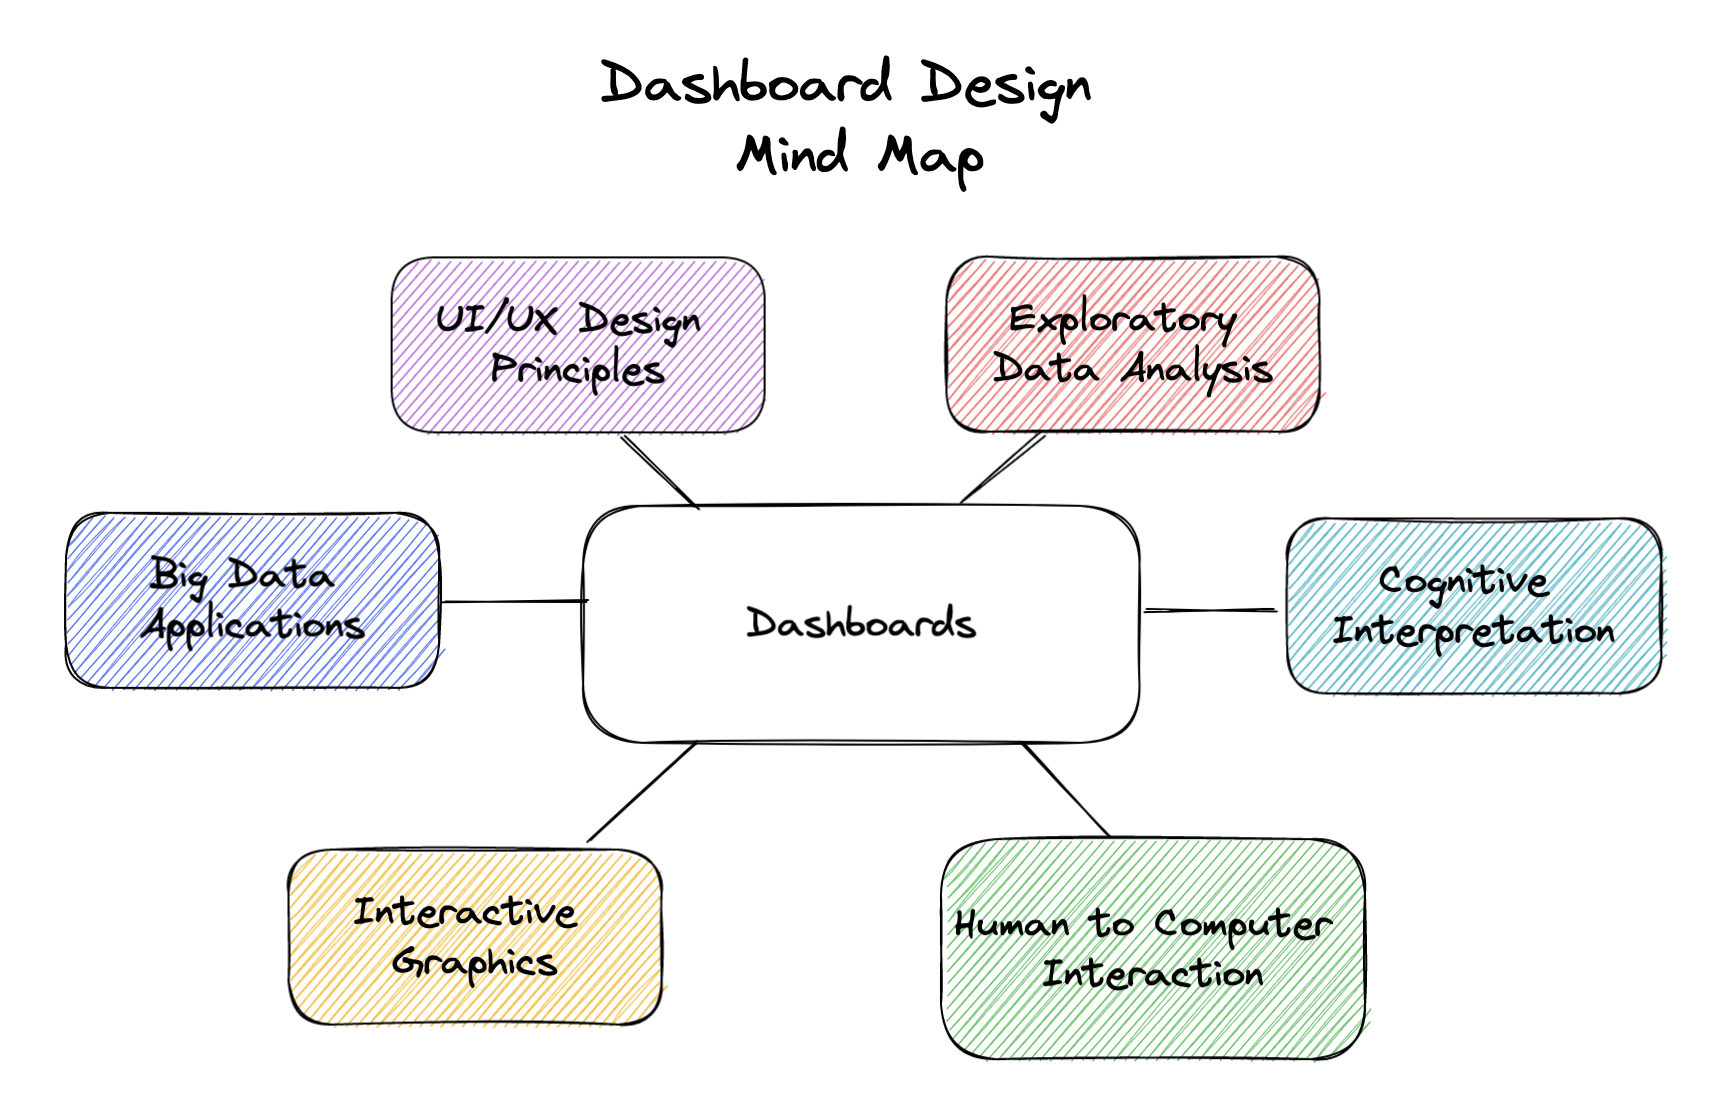
\includegraphics[width=\textwidth]{figure/DashboardDesignMap}
\captionof{figure}{Dashboard Design Mind Map}
\end{center}

Dashboard Design in combination of naive users with adding new graphical visualization testing the effectiveness of new graphic.

Data Visualizations can be described as a graphical representation of tabular data and information. Data visualization tools are used in ways to accessible way to see and understand trends, outlines, and patterns in data.

The literature review will explore the facets of Exploratory Data Analysis (EDA) through the history of graphical representation followed by the review of Dashboard Design and Visual Information.

Roles of graphics in Data Analysis:
Graphics and Tables are forms of communication that we are looking to determine:

\begin{itemize}
\tightlist
\item
  What is the audience?
\item
  What is the message?
\end{itemize}

Analysis: design to see patterns, trends, and the process of data description, interpretation
Presentation: design to attract attention, make a point, illustrate a conclusion

Based on the following diagram

\begin{center}
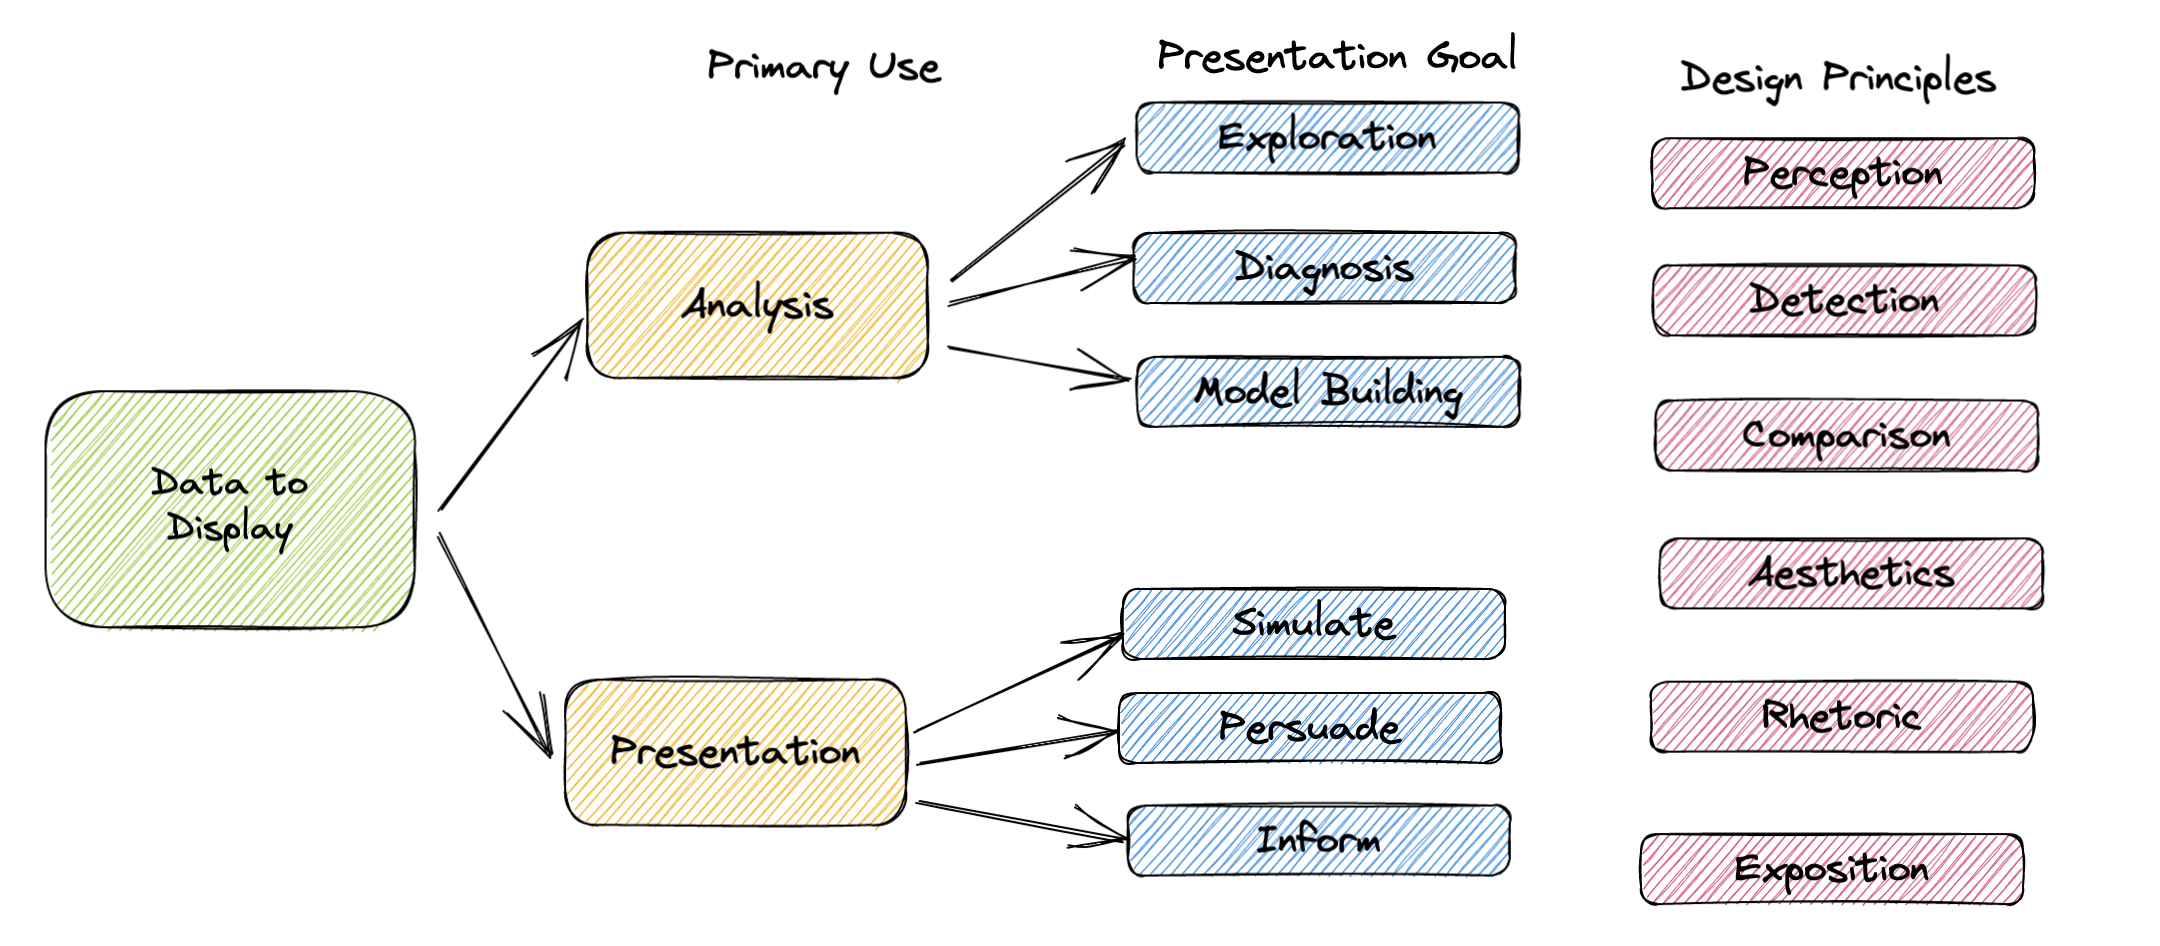
\includegraphics[width=\textwidth]{figure/RolesofGraphics}
\captionof{figure}{Roles of Graphics}
\end{center}

As tabular data grows in our society that has pushed our needs to create visualizations that represent that data in a correct and digestible way. The work that has been done in statistical graphical research would suggest that the work that is done in this work has grown increasing in formal adding sound guidelines with statistically sound metrics that are needed. This work has been explored in various disciplines but not in a statistical graphics. We know that dashboards are visual information tools that include and have multiple statistical graphics. Thus, we should consider and think about the fact that we may need to consider the statistical and psychological framework in a dashboard that will combine multiple statistical graphics.

One graphic can be misleading alone, but can a two graphics together be considered misleading when placing two ``correctly'' design graphics together on a dashboard. This is something that visual information researchers explore but don't test.

Since, we don't completely understand the way that basic statistical graphics are

When effectively adding advance graphical representations to a naive user, what have we done to create a true understanding to an engaging idea of what's going on.

\hypertarget{history-of-exploratory-data-analysis-eda}{%
\section{History of Exploratory Data Analysis (EDA)}\label{history-of-exploratory-data-analysis-eda}}

Visualizations of data are important for exploratory data analysis (EDA) along with model diagnostics. Plots for EDA are a useful tool for guiding an analyst in discovering the relationships between variables in their data. In the case when using plots in model diagnostics, plots help analysts determine whether or not the model is appropriate way to model. During the initial EDA stage, an analyst may find that a variable or a covariate is directly related to the dependent variable when looking at a correlation heatmap or a scatterplot. This will be important to know before starting a linear model analysis. Much of our general understanding is from introductory statistics courses. The basic understanding can be formalized in a way that will visual discovery process.

\hypertarget{study-1-eda-through-the-eyes-of-tukey}{%
\subsection{Study 1: EDA through the eyes of Tukey}\label{study-1-eda-through-the-eyes-of-tukey}}

John Tukey was the first to organize the collection and methods associated philosophy into the Exploratory Data Analysis (EDA). Tukey was a person who helped utilize the likes of stem-and-leaf plot, boxplot resistant smooth and rootgram.

Tukey's Principles in EDA:

\begin{enumerate}
\def\labelenumi{\arabic{enumi}.}
\tightlist
\item
  \emph{Revelation}: Graphical exploration looking for patterns or displaying fit.
\end{enumerate}

\begin{itemize}
\tightlist
\item
  The method is used to demonstrate things about data that are not understood by a single numeric metric. This has been useful in the ideology of graphing the data before you develop summary statistics.
\end{itemize}

\begin{enumerate}
\def\labelenumi{\arabic{enumi}.}
\setcounter{enumi}{1}
\tightlist
\item
  \emph{Resistance}: describing the general patterns of the data.
\end{enumerate}

\begin{itemize}
\tightlist
\item
  This step should be insensitive to outliers. In general thinking about the types of resistant measures (i.e.~median or mean).
\item
  This step is making sure to determine data patterns.
\end{itemize}

\begin{enumerate}
\def\labelenumi{\arabic{enumi}.}
\setcounter{enumi}{2}
\item
  \emph{Reexpression}: the natural scale/state that the data are at their best. This will be the step at which the scale of data can be useful for analysis. The reexpressing data to a new scale by taking the square root or logarithmic scale.
\item
  \emph{Residual}: the mostly known parts of EDA but is done in the way of accessing fit of the data. This is taught in every statistics 101 class. The growth of machine learning and prediction methods have now used residuals more in the tool box to access best prediction models.
\end{enumerate}

\begin{itemize}
\tightlist
\item
  The idea generally is to determine the deviations in the data from a general pattern looking at the data from the fit of the data.
\end{itemize}

\hypertarget{study-2-eda-through-the-eyes-of-the-modern-grammar-of-graphics-wickham-etc.}{%
\subsection{Study 2: EDA through the eyes of the modern grammar of graphics (Wickham, etc.)}\label{study-2-eda-through-the-eyes-of-the-modern-grammar-of-graphics-wickham-etc.}}

The grammar of graphics (gg of ggplot2) is a theory that is well-defined for creating statistical graphics with work from Wilkinson (\textbf{Wilkinson1999?}) and Hadley Wickham (Wickham, 2016). Leland Wilkinson originally created the structure and defined the phrase. Grammar of graphics is defined as the framework which follows a layered approach to describe and construct visualizations or graphics in a structured manner.

\begin{center}
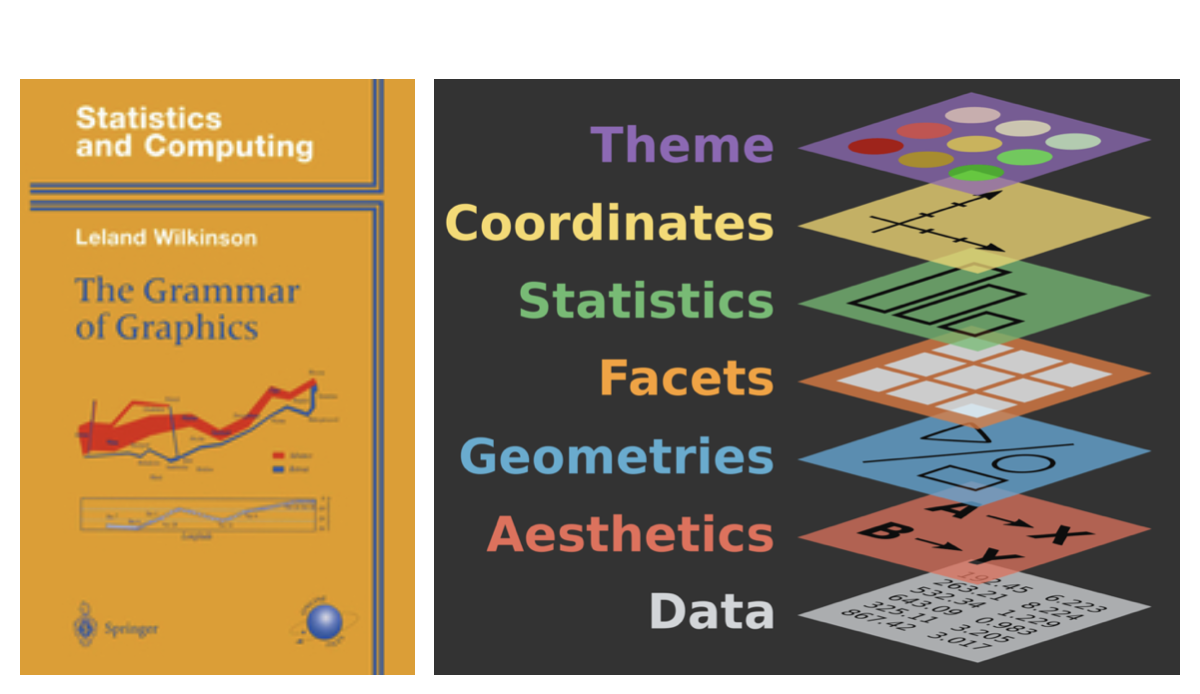
\includegraphics[width=\textwidth]{figure/ggDiagram}
\captionof{figure}{Grammar of Graphics Diagram of Wickham and Wilkinson's work}
\end{center}

The theory of graphics are based on plot layers, which is built with four distinct pieces:

\begin{itemize}
\tightlist
\item
  the data
\item
  aesthetic mapping - \emph{takes data and maps the variable in the data frame to a particular visual features}
\item
  statistical transformation - \emph{determines how to transform the data to values to create the visual feature}
\item
  geometric object and a position adjustment - \emph{geom object is used to draw a plot layer and position adjustment is to help with adjusting the visual feature in the space.}
\end{itemize}

There are seven major components that help build effective visualizations that build on one another. There are seven major components that help build effective visualizations. The following diagram will display the

\begin{center}
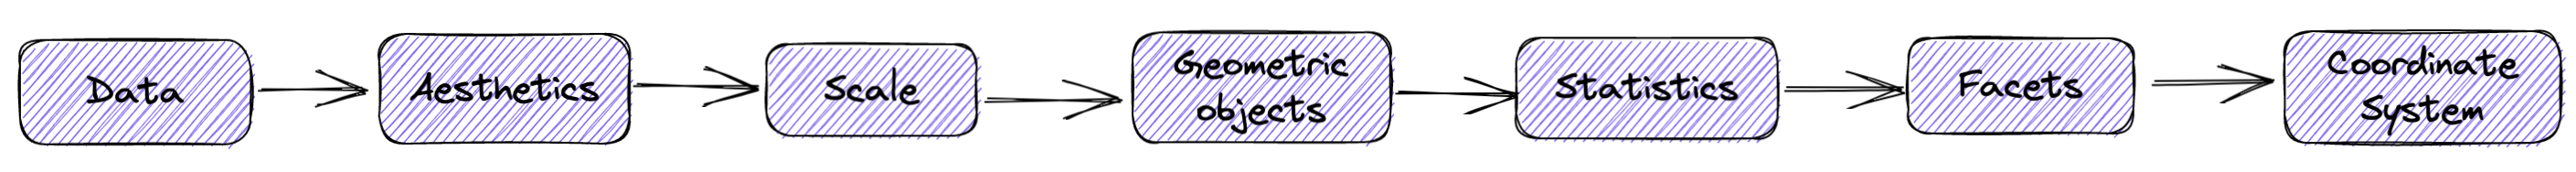
\includegraphics[width=\textwidth]{figure/EffectiveDataGraphics}
\captionof{figure}{Effective Data Graphics}
\end{center}

\begin{itemize}
\tightlist
\item
  Data
\item
  Aesthetics
\item
  Scale
\item
  Geometric Objects
\item
  Statistics
\item
  Facets
\item
  Coordinate system
\end{itemize}

\hypertarget{study-3-eda-through-the-eyes-of-big-data-di-cook-etc.}{%
\subsection{Study 3: EDA through the eyes of Big Data (Di Cook, etc.)}\label{study-3-eda-through-the-eyes-of-big-data-di-cook-etc.}}

Big Data Analytics is where advanced analytic techniques are applied on big data sets.
- Analytics based on large data samples reveals and leverages business change.
The larger the set of data, the more difficult it becomes to manage.

\hypertarget{characteristcs-of-big-data}{%
\subsubsection{Characteristcs of Big Data}\label{characteristcs-of-big-data}}

\begin{center}
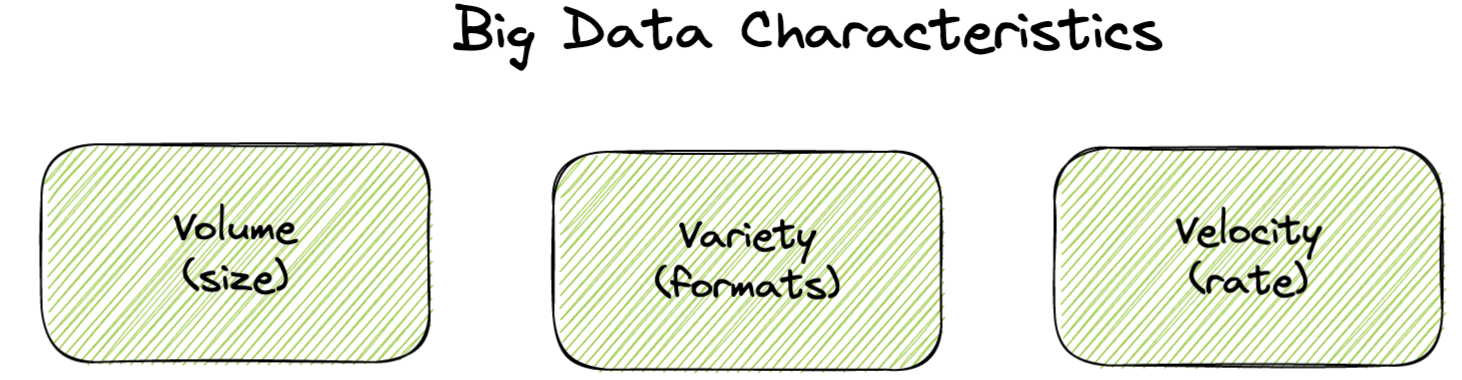
\includegraphics[width=\textwidth]{figure/BigDataDiagram}
\captionof{figure}{Big Data Diagram}
\end{center}

There are three main features characteristics of big data:
- Volume: is its size and how enormous it is
- Variety: includes the different formats and types of data, as well as the different kinds of uses and ways if analyzing the data
- Velocity: refers to the rate with which data is changing, or how often it is created

\hypertarget{big-data-storage-and-management}{%
\subsubsection{Big Data Storage and Management}\label{big-data-storage-and-management}}

Where and how this data will be stored once it is acquired:
- Traditional methods of structured data storage and retrieval include relational databases, data marts, and data warehouses.
- Uploaded to the storage from operational data stores using: Extract, Transform, Load (ETL) or Extract, Load, Transform (ELT) tools which extract data from outside sources, transform the data to fit operational needs, and transformed and cataloged before made available for data mining and online analytical functions.

Given the growing numbers of data sources as well as the sophistication of data analyses, big data storage should allow analysts to easily produce and adapt data rapidly.

\begin{itemize}
\tightlist
\item
  This requires an agile database, whose since current data analyses use complex statistical methods, and analysts need to be able to be deep and serve as a sophisticated algorithmic run time engine.
\end{itemize}

A list of Data Visualizations Types can be broken down into the following:

\begin{itemize}
\tightlist
\item
  Tables (Pivot Tables)
\item
  Line Chart or Line Graph
\item
  Bar Chart
\item
  Scatter Plot
\end{itemize}

\hypertarget{applications-of-data-visualization-types}{%
\section{Applications of Data Visualization Types}\label{applications-of-data-visualization-types}}

\hypertarget{tables}{%
\subsection{Tables}\label{tables}}

A table is defined as set of objects or individuals divided by intersecting components, which produces a data table or tabular data. A table will allow for a reader to perceive information at a high level in its totality.

\hypertarget{line-chart-line-graphs}{%
\subsection{Line Chart (Line Graphs)}\label{line-chart-line-graphs}}

A line chart is defined as a graph that uses lines to connect individual data points. A line graph displays quantitative and qualitative variables of tabular data (tidy data).

\hypertarget{bar-chart}{%
\subsection{Bar Chart}\label{bar-chart}}

A bar chart is defined as a chart that compares different categories of data using rectangular bars that represent the value of tabular (tidy) data.

\hypertarget{scatter-plot}{%
\subsection{Scatter Plot}\label{scatter-plot}}

A scatter plot is defined as a graph in which the values of two variables are plotted along two axes, the pattern of the resulting points revealing any correlation present.

\hypertarget{historyreview-of-graphical-representation}{%
\section{History/Review of Graphical Representation}\label{historyreview-of-graphical-representation}}

\hypertarget{historyorigin-of-statistical-visualization}{%
\subsection{History/Origin of statistical visualization}\label{historyorigin-of-statistical-visualization}}

Visual inference uses our ability to detect graphical anomalies. The idea of formal testing remains the same in visual inference -- with one exception: The test statistic is now a graphical display which is compared to a ``reference distribution'' of plots showing the null.\href{}{REFERENCE WEBSITE}

\hypertarget{overview-of-tables-and-graphics-in-papers}{%
\subsection{Overview of tables and graphics in papers}\label{overview-of-tables-and-graphics-in-papers}}

\hypertarget{advancement-of-graphical-visualizations-in-dashboards}{%
\subsection{Advancement of graphical visualizations in dashboards}\label{advancement-of-graphical-visualizations-in-dashboards}}

Visualizations have become more effective in more recent years due to the pandemic and the Johns Hopkins University COVID-19 Dashboard (Dong E, 2022) \href{https://coronavirus.jhu.edu/map.html}{Dashboard}, for most of the world, we were glued to our computers, TVs and phones. As a result, we watched as the dashboard changed in real time to adapt to the needs of the users. In part to data growing and changing, the dashboard as well as the visualizations were needed in a condense platform. The need to be concise along with vastly informative can be a bit of a struggle when it comes to data visualizations. The human brain is capable of only taking in a set amount of data at a time from a table or a paragraph. The space of infographics have been a much better way of looking at data on a creative scale. While this may be a way of seeing the data in a nice way, infographics miss the interactive piece about data that many people would like to explore.

\hypertarget{applications}{%
\subsection{Applications}\label{applications}}

Two general applications in areas of visual inference have developed since the work of (Buja et al., 2009). These applications are actual methodology and methodology based on protocols. Actual methodology applications are used with alternative and corresponding null hypotheses, which perform visual inference tests to show many participants of different backgrounds with lineups.

\hypertarget{dashbaord-design-human-perception-visual-information}{%
\section{Dashbaord Design/ Human Perception (Visual Information)}\label{dashbaord-design-human-perception-visual-information}}

\hypertarget{historyorigin-of-dashbaord-design}{%
\subsection{History/Origin of Dashbaord Design}\label{historyorigin-of-dashbaord-design}}

Formally, a dashboard is a visual display of the most important information needed to achieve one or more objectives; consolidated and arranged on a single screen so the information can be monitored at a glance.(Few, 2006). As dashboard has particular characteristics:

\begin{itemize}
\tightlist
\item
  Achieve specific objectives
\item
  Fits on a single computer screen
\item
  Information can be displayed in multiple mediums (web browser or mobile device)
\item
  Can be used to monitor information at a high level
\end{itemize}

While a dashboard can be extremely useful, it may be worth describing that a poorly designed dashboard will not be used. A dashboard should be concise, clear, and intuitive when displaying components in combination of with a customized list of requirements of users.

Much of the work done within statistical research and dashboard design has to do with collaboration with other academic researchers. While this may be the best for the growth of the discipline, one will find that working with collaborators with the

A collaboration is defined when 2 or more entities work together to produce a desired and shared outcome. Interdisciplinary research with collaboration is a pinnacle aspect of dashboards and statistical graphics to produce innovation and scientific knowledge.

The National Academies defines research collaboration as follows (NATIONAL ACADEMY OF SCIENCES, NATIONAL ACADEMY OF ENGINEERING,AND INSTITUTE OF MEDICINE OF THE NATIONAL ACADEMIES, 2004):

\begin{quote}
Interdisciplinary research (IDR) is a mode of research by teams or individuals that integrates information, data, techniques, tools, perspectives, concepts, and/or theories from two or more disciplines or bodies of specialized knowledge to advance fundamental understanding or to solve problems whose solutions are beyond the scope of a single discipline or field of research practice.
\end{quote}

\hypertarget{section-8-historyorigin-of-human-perception-of-statistical-graphics}{%
\subsection{Section 8: History/Origin of Human Perception of Statistical Graphics}\label{section-8-historyorigin-of-human-perception-of-statistical-graphics}}

The human perception plays a direct role in the area of visualizations. The human perception importance was cited by the NSF panel on graphics and image processing that proposed the ``scientific visualization'' (\textbf{NSF?}).

Data Analysis tasks closely resemble the cognitive process known as sensemaking. Tukey and Wilk (John W. Tukey \& Wilk, 1966) highlight the role of cognitive processes in their initial descriptions of EDA.

\begin{quote}
The basic general intent of data analysis is simply stated: to seek through a body of data for interesting relationships and information and to exhibit the results in such a way as ro make them recognizable to the data analyzer.
\end{quote}

Mallows and Walley (Mallows \& Walley, 1980) list psychology as on of four areas likely to support a theory of analysis. Data analyses rely on the mind's ability to learn, analyze, and understand. Assigning meaning is not a statistical or computational step, but a cognitive one. Each data analysis is part of a larger, cognitive process.

Untrained analysts can and do ``analyze'' data with only their natural mental abilities
- The mind performs its own data analysis - like process to create detailed understandings of reality from bits of sensory input.

\hypertarget{schemas-and-sensemaking}{%
\subsubsection{Schemas and Sensemaking}\label{schemas-and-sensemaking}}

Cowan (Cowan, 2001) suggested that the average person can only hold two to six pieces of information in their attention. People are able to develop detailed understandings of reality, which is infinitely complex.

Cognitive structures consists of mental models and their relationships ((Rumelhart \& Ortony, 1976), (Carley \& Palmquist, 1992), (\textbf{jonassen1996?})). mental models have been studied under a number of different names.

\begin{center}
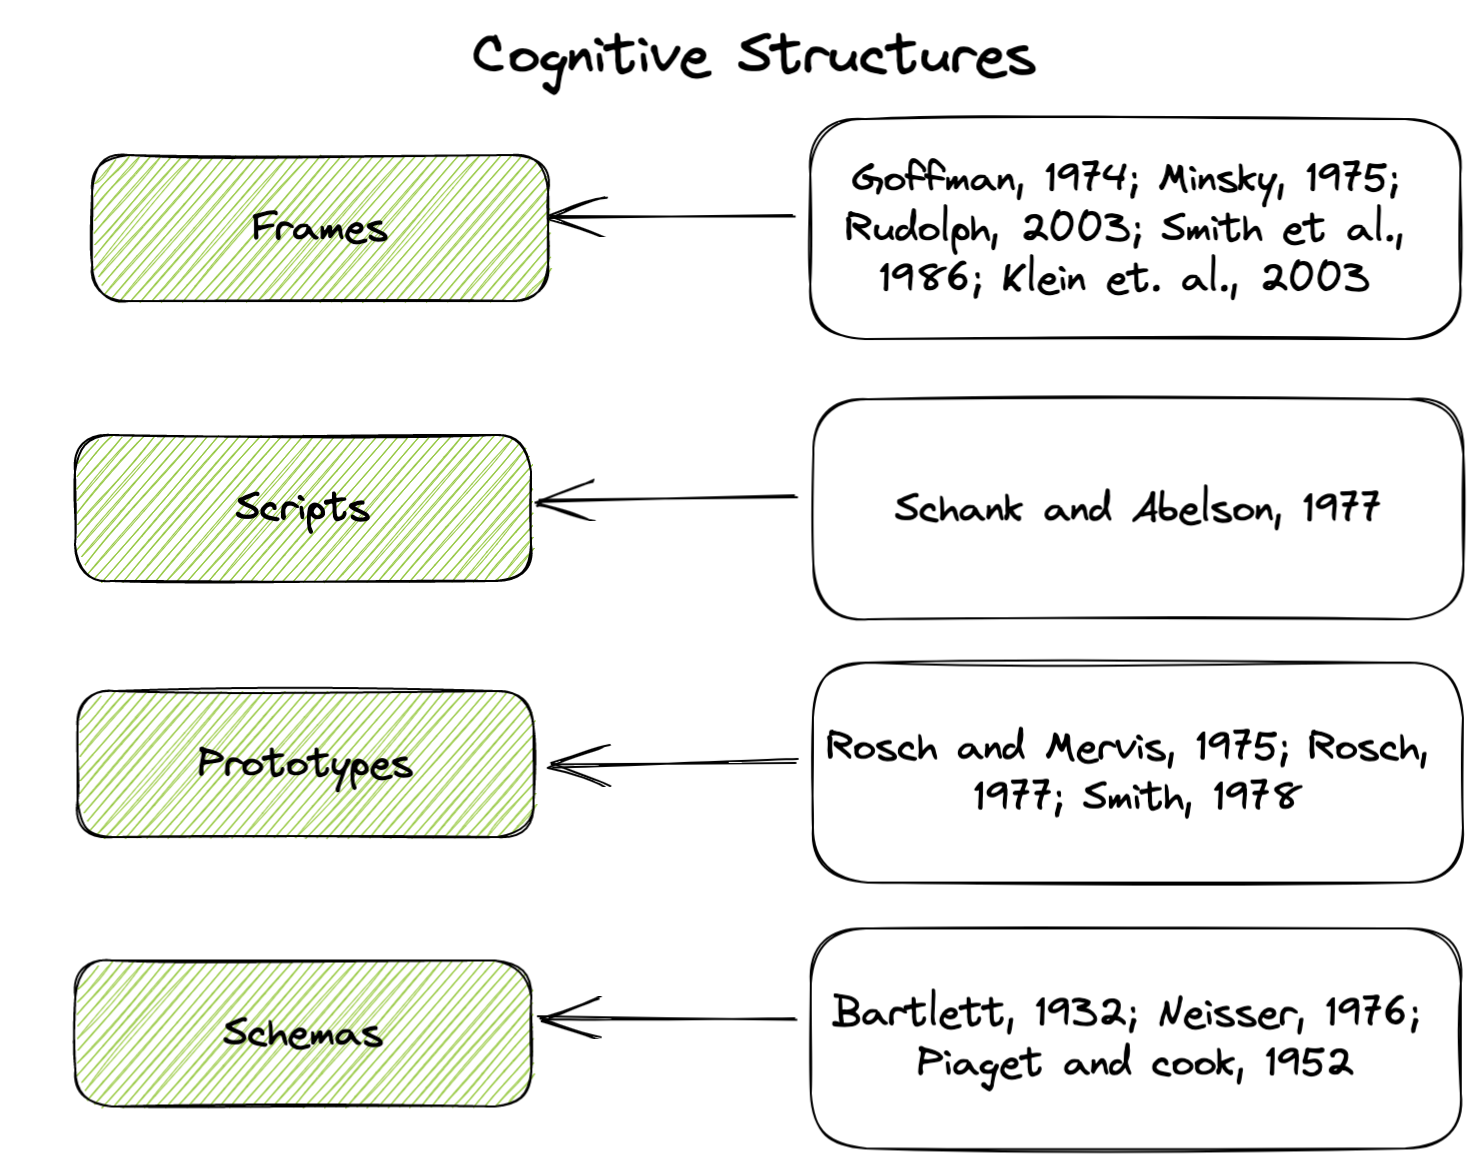
\includegraphics[width=\textwidth]{figure/CognitiveStructuresCitationTimeline}
\captionof{figure}{Cognitive Structures Citation Timeline}
\end{center}

A schema is a mental model that contains a breadth of information about a specific type of object or concept. Schemas are organized into semantic networks based on their relationships to other schemas (Wertheimer, 1938), (Rumelhart \& Ortony, 1976). This arrangement helps the brain process its experiences instead of storing every sensory observation, the brain only needs to maintain its schemas, which are sufficient summarizes of all previous observations. Some ``memories'' may even be complete recreations built with a schema (Bartlett \& Remembering, 1932), (Klein, Phillips, Rall, \& Peluso, 2007)

\hypertarget{study-9-dashbaord-design-in-regards-to-human-perception}{%
\subsection{Study 9: Dashbaord Design in regards to Human Perception}\label{study-9-dashbaord-design-in-regards-to-human-perception}}

Data Scientists and Statisticians have produced more graphics since the start of the pandemic. The reasons why someone will create a graphic or dashboard may include, but not limited to: understanding raw data structures, in order to analyze model assumptions and present predictions along with display of key performance metrics of business logic. These goals help work to navigate are best served by quick-and-dirty representations of the data, while highly polished graphics may be more useful in other situations. It is useful and important to correctly convey data meaning that we need to understand how graphics are perceived on a dashboard on a general level. As previous research done by Tukey focused on graphics as a tool for exploratory analysis. Tukey describes in Exploratory Data Analysis (John W. Tukey, 1977) that pictures are often used to display data in a more enhanced version than a table. Tukey outlines detail types of different graphics and at which situations to utilize these graphics. The article - ``External cognition: how do graphical representations work?'' by Scaife and Rogers critique the disparate literature on graphical representations, focusing on four representative studies. In general, this will help in the framework of psychology of the perceptual experience.

The visual reference model developed by Card et al. (S. K. Card \& Shneiderman, 1999) describes and identifies the three phases of the visualization process.

\begin{center}
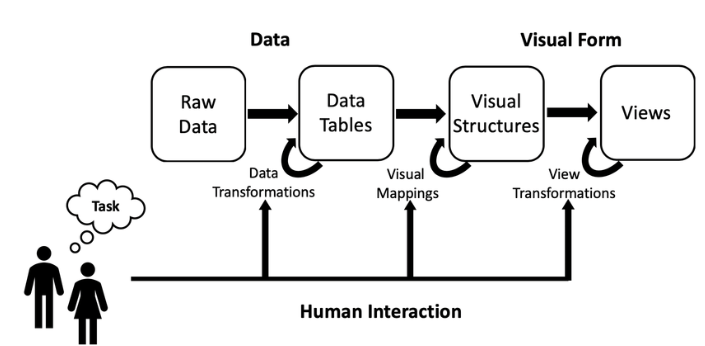
\includegraphics[width=\textwidth]{figure/VizModelDiagram}
\captionof{figure}{Visual Reference model by Card}
\end{center}

While the External Cognition describes the advances in graphical technology and how little had been done in the work of the cognitive framework of the discipline, the following citations by Ware are attempting to develop the necessary guidelines that are useful for the work done by the perceptual experience.

Colin Ware ``Information Visualization: Perception for Design'' (Ware, 2004) there are four stages of visualization
- The collection and storage of data itself
- The preprocessing design to transform the data into something we can understand
- The display hardware and the graphics algorithms that produce the image to screen.
- The human perceptual and cognitive system

The overlapping understanding in the field, while Ware takes the process one step further to not just allow the end user to understand the outcomes but to curate the outcomes with a visual perception of the data that makes the cognitive load easier for the end-user.

A dashboard has a multitude of information related to tabular data from multiple sources. Design should be recorded a produced with content that will allow for reproducibility. A dashboard should have some content related to interaction from the user. This interaction can be in multiple forms: toggling through the selection of variables to display uniformly to the use of interaction on the graph. Allowing a user to best understand what is being displayed in the graph.

The entire dashboard/Interface should have a human perception piece that is useful for the user to comprehend and use. If the user is visually overwhelmed, then the dashboard/interface is not useful.

\begin{itemize}
\tightlist
\item
  Identified the highly relevant from dashboard design perspective (O'Donnell \& David, 2000)
\end{itemize}

\begin{enumerate}
\def\labelenumi{\arabic{enumi}.}
\tightlist
\item
  Interaction and feedback given by information systems
\item
  Type of presentation format to be used
\item
  Differences in the amount of information load.
\end{enumerate}

Information load is an important issue, as dashboards need to provide the right amount of decision cues, without overwhelming the user with excess information.

``A decision cue is a feature of something perceived that is used in the interpretation of perception (Choo, 2009),'' where perception is an inferential process as objects in the environment can only be perceived indirectly through available information that has been sensed by the individual (Brunswik, 1952).

Visual complexity and information utility is required. Visual complexity refers to "degree of difficulty in providing a verbal description of an image.Olivia, Mack, Shrestha, \& Peeper (2004)

\begin{itemize}
\tightlist
\item
  Graphs are more suitable for spatial tasks (ex. for comparing a set of values) (Vessey \& Galletta, 1991),(Umanath \& Vessey, 1994); (Vessey, 1994)
\item
  Graphs reduced the negative influence of information overload
\item
  Graphs produced better correlation estimates and decreased time on task (\textbf{schulzand?} ; Booth \& Siegler, 2006)
\item
  Self organizing maps and multidimensional scaling did not significantly outperform tabular representations (Huang et al., 2006)
\end{itemize}

The purposes of a dashboard:

\begin{enumerate}
\def\labelenumi{\arabic{enumi}.}
\tightlist
\item
  Consistency
\item
  Monitoring
\item
  Planning
\item
  Communication
\end{enumerate}

``Use of interactive visual representations of abstract, non physically based data to amplify cognition.'' (Card, Mackinlay, \& Shneiderman, 1999)

Visual perception involves two elements - the perceptual and conceptual gist. The perceptual gist refers to the process of the brain when it determines the image properties that provide the structural representation of a scene, like color and texture. The conceptual gist refers to the meaning of the scene, which is improved after the perceptual information is received. (Friedman, 1979; Olivia, Mack, Shrestha, \& Peeper, 2004)

Visual complexity might increase with the quality and range of objects as well as with varying material and surface styles (Heylighen, 1997).

Repetitive and uniform patterns and existing knowledge of the objects in the scene reduce visual complexity (Olivia, Mack, Shrestha, \& Peeper, 2004)

Guidelines for new generation dashboards refer to:
1. Aligning business processes with latest information to provide business intelligence at all levels in the company.
2.Using intuitive and easy to digest visuals for delivering information to busy executives.
3. Sound Navigation
(\textbf{ZiffDavisEnterprise2008?})

If the guidelines on our visual information load can be related back to statistical terminology, we can consider this the fisher information of visual information load. This load can be used as a metric of balancing the amount of information and not over load the consumer.

Visual Data Mining

For data mining to be effective, it is important to include the human in the data exploration process and combine the flexibility creativity and general knowledge of the computational power of today's computers. Visual data exploration aims at integrating the human in the data exploration process, applying its perceptual abilities, to the large data sets available in today's computer systems.(Keim, 2002)

The visual data exploration process can be seen as a hypothesis generation process:
- The visualizations of the data allow the user to gain insight into the data and come up with new hypotheses
- Along with verification of the hypotheses

The main advantages of visual data exploration over automatic data mining techniques from statistics or machine learning are:
- visual data exploration can easily deal with highly inhomogeneous and noisy data.
- visual data exploration is intuitive and requires no understanding of complex mathematical or statistical algorithms or parameters.

Visual Exploration Paradigm also known as MGV (Massive Graph Visualizer), an integrated visualization and exploration system for massive multidigraph navigation.(Abello \& Korn, 2002). MGV usually follows a three step process:
- overview first
- zoom and filter
- details-on-demand

The user identifies interesting patterns and focuses on one or more of them. Note that visualization technology does not only provide the base visualization techniques for all three steps but also bridges the gap between the steps.

Visualization Technique Classification:
- Standard 2D/3D displays such as bar charts and x-y plots
- Geometrically transformed displays, such as landscapes and parallel coordinates as used in a scalable framework
- Icon-based displays such as needle icons and star icons as used in MGV
- Dense pixel displays such as the recursive pattern and circle segments techniques and the graph sketches as used in MGV
- Stacked displays, such as treemaps or dimensional stacking

Interaction and distoration techniques allow users to directly interact with the visualizations.
- Projection as used in the Grand Tour System
- Filtering as used in Polaris
- Zooming as used in MGV and scalable framework
- Linking and Brushing as used in Polaris and the scalable framework

Design Theory in Information System

The knowledge is distinguished as the fifth of five types of theory:
1. Analyzing \& describing
2. Understanding
3. Predicting
4. Explaining and predicting
4. Design and action

A definition of information systems suitable for our purposes is that it concerns: "the effective design delivery use and impact of information technology in organizations and society (\textbf{Avison?}).

The two paradigms characterize much of the research in the Information systems discipline:
- \emph{Behavioral Science Paradigm} - seeks to develop and verify theories that explain or predict human or organizational behavior (roots in natural science research methods).
- \emph{Data Science Paradigm} - seeks to extend the boundaries of human and organizational capabilities by creating new and innovative artifacts (roots in engineering and the sciences of the artificial).(\textbf{simon1996?})

Technology and behavior are not dichotomous in an information system. They are inseparable (\textbf{lee2000?}). Information technology (IT) artifacts are broadly defined as:
- constructs (vocabulary \& symbols)
- models (abstractions \& representations)
- methods (algorithms \& practices)
- instantiations (implementated \& prototype systems)

These are concerte prescriptions that enable IT researchers and practitioners to understand and address the problems inherent in developing and successfully implementating information systems within organizations ((\textbf{march1995?}); (\textbf{Nunamaker1991?})).

\#\#\# Interactive Visualization in Exploratory Data Analysis (EDA)

Data Scientists and other analytic professionals often use interactive visualization in the dissemination phase at the end of a workflow during which findings are communicated to a wider audience. Digital tools are critical to data science and analytics workflows and current practice spans across the following:
- \emph{Data Analysis Tools} - R, Pandas and SAS
- \emph{Data Warehousing Services} - MySQL, MongoDB, or Amazon Redshift
- \emph{Machine Learning Libraries} - scikit-learn o Apache MLlib

A common process typically consists of the following general stages:
1. \emph{Discovery}: Formulating an interesting question and determining the data necessary to answer it.
2. \emph{Acquisition}: Locating, organizing and preparing data so that it is accessible to the chosen analysis environment.
3. \emph{Exploration}: Investigating and analyzing the data set in order to collect insights and understand the data
4. \emph{Modeling}: Building fitting and validating a model that can explain the data set and the observed phenomena
5. \emph{Communication}: Disseminating the results to stakeholders in reports, presentation and charts.

Static Visualization is commonly used in the communication phase of data science workflows and data scientists sometimes use them as part of the analysis as well. John Tukey's EDA methods are those that are known ad well vetted in the field currently. However, (\textbf{Satyanarayan?}) began to address this by introducing a high-level grammar of graphics, called ``Vega-Lite,'' which presents a set of standardized linguistic rules for producing interactive information visualizations using a concise JSON format for data to be represented by the grammar. Vega-Lite has been directly implemented in R via the \texttt{ggvis} package using the same - albeit slightly lower-level.

Contextual Design

(\textbf{wixon?}) introduce ``contextual design'' as a systems development method in which the researcher partners with the user at the user's place of work to ``develop a shared understanding'' of the user's activities, and they define contextual inquiry as the first part of the broader process. Contextual inquiry is the data collection step of the field research element of the contextual design method, and it emphasizes four essential principles:

\begin{enumerate}
\def\labelenumi{\arabic{enumi}.}
\tightlist
\item
  The context of the sctivity being performed by the user
\item
\end{enumerate}

\hypertarget{ggpcp-package---generalized-parallel-coordinate-plots}{%
\section{\texorpdfstring{\texttt{ggpcp} package - Generalized Parallel Coordinate Plots}{ggpcp package - Generalized Parallel Coordinate Plots}}\label{ggpcp-package---generalized-parallel-coordinate-plots}}

\hypertarget{parallel-coordinate-plot-visualization-review}{%
\section{Parallel Coordinate Plot Visualization Review}\label{parallel-coordinate-plot-visualization-review}}

Parallel coordinate plots have been implemented in analysis software since the mid 1980s ((Inselberg, 1985), (Wegman, 1990)). Parallel Coordinate Plot Visualization, also called parallel plot, is an established field of high dimensional visualization of xy coordinate analysis. Parallel coordinate plots have such a unique structure that will allow for data structures with n-dimensions. As data grows in exploratory data analysis, the use of data visualizations will be more important and useful to understanding the underlying structures of useful data for analyses. Several packages in R are dedicated to visualizing parallel coordinate plots.

Dashboards can be used to help understand and support many types of data in any set of business objectives that are important. There are many different ways to label and utilize dashboards into different types.

Dashboards are cognitive tools that should be used to improve understanding of data, which should help people visually find relationships, trends, patterns and outliers. Most importantly, dashboards should leverage people's visual cognitive capabilities.

\hypertarget{parallel-coordinates-in-eda}{%
\subsection{Parallel Coordinates in EDA}\label{parallel-coordinates-in-eda}}

EDA refers to methods and procedures for exploring the data space to learn about a data set and so, by analogy, exploratory modeling analysis (EMA) refers to methods and procedures for exploring the space of models, which may be fit, to a data set.

Interactive graphics are excellent for EDA, they are designed for exploring rather than presenting information (and more) can be obtained by directly querying the graphic (Unwin, Volinsky, \& Winkler, 2003).

\begin{itemize}
\tightlist
\item
  PCPs enable the display of multi-dimensional data in two-dimensional space.
\item
  There must be some loss of information but this can be partly counteracted by varying the order of the axes.
\item
  Interactivity is valuable for reordering the axes flexible and fast.
\item
  Interaction is valuable for dealing with the dense mass of lines produced by large data sets.
\end{itemize}

Being able to select subgroups of cases, highlight the selected lines, switch between different subgroups, all assist in interpreting the other wise intricate displays which arise.

\hypertarget{r-packages}{%
\subsection{R Packages}\label{r-packages}}

There are R packages that exist for Parallel coordinate plots, with some built-in functionality, but not many exist for advance exploratory data analysis visualizations. Beginning with base plot package \texttt{parcoord} developed in MASS by (\textbf{Venables?} and Ripley 2004). The package is limited by extensive, in which it contains more than methods for the parallel coordinate plot visualization. It contains the following tools for 2D visualization of PCPs. Another package \texttt{gclus} was developed by (Hurley, 2019) implements \texttt{cparcoord} to include panel color of the strength of a correlation between neighboring axes.

While base R packages are useful, there are a few packages within the ggplot2 environment implementing parallel coordinate plots. With ggplot2 extension packages, the theory of grammar of graphics are at the focal point of plots. The following packages (Schloerke et al., 2021) and \texttt{ggpcp} are built with the fundamental guidelines for graphic literacy for numeric variables. \texttt{GGally} was originally designed for the following pieces of the graphic design: \href{}{LIST THE PACKAGE'S STARTING PLANS}, so it also contains much more capabilities for PCPs with addition to visualizations. \texttt{ggpcp} we separate the data transformations from the visualization, i.e.~rather than working with a single function to draw a plot, we are providing a set of functions that work together (Hofmann, VanderPlas, \& Ge, 2022).

\texttt{ggparallel} implements and combines different types of parallel coordinate plots for categorical data: hammock plots, parallel sets plots, common angle plots, and common angle plots with a hammock-like adjustment for line widths (Hofmann \& Vendettuoli, 2013b).

\hypertarget{ggpcp-package-importance}{%
\subsection{\texorpdfstring{\texttt{ggpcp} package importance}{ggpcp package importance}}\label{ggpcp-package-importance}}

As mentioned in previous sections, that parallel coordinate plots has a long line of history. However, we are now looking to incorporate the use of categorical data. The \texttt{ggpcp} implements the Grammar of graphics and the principled manor of categorical variables. This package separates the data managing part from the plots by giving full access to the users while keeping the number of parameters manageably law. (Hofmann, VanderPlas, \& Ge, 2022)

While the \texttt{ggpcp} package is the first iterations of the package can be changed in the way that will allow for the user to rearrange the variables on the y-axis, this use can be helpful so that someone will be able to understand better. When we look at graphics, through the eyes of someone that is not use to a graphic, we can see the usefulness and effectiveness of allowing more interaction from the user. This consideration is one that will be exhausted in my work. We will explore the ways at which one level of interaction from the user can create a better plot for understanding.

\hypertarget{conclusion}{%
\section{Conclusion}\label{conclusion}}

\hypertarget{rmd-basics}{%
\chapter{Chapter Paper on Rural Shrink Smart Manuscript submitted to Journal of Data Science Special Issue}\label{rmd-basics}}

\hypertarget{abstract}{%
\section{Abstract}\label{abstract}}

Many small and rural places are shrinking. Interactive dashboards are the most common use cases for data visualization and context for exploratory data tools. In our paper, we will explore the specific scope of how dashboards are used in small and rural area to empower novice analysts to make data-driven decisions. Our framework will suggest a number of research directions to better support small and rural places from shrinking using an interactive dashboard design, implementation and use for the every day analyst.

\hypertarget{introduction-1}{%
\section{Introduction}\label{introduction-1}}

As the amount of data has increased in nearly every facet of life, the need to make sense of that data in an approachable, accessible form has become ever more important.
As a result, many companies and organizations use interactive dashboards to present these data in a more useful and visually appealing form (Sarikaya, Correll, Bartram, Tory, \& Fisher, 2019).

In many cases, dashboards support viewers' information processing, helping to make sense of complex data, navigate through a dataset, and supporting decision making based on the data.

Dashboards are often used, as with the car display of the same name, to provide summary information about many separate attributes of a common entity. One glance at a car's dashboard will tell you the speed, RPM, engine temperature, amount of gas in the tank; more importantly, however, the goal is not for the user to remember all of these characteristics, but to assess whether any of these quantities is outside of the expected range.
Similarly, interactive dashboards for data are often used to display many different attributes and performance metrics which are of importance for stakeholders.

In this paper, we discuss the process of designing a dashboard to present publicly available government data to stakeholders in small Iowa towns to facilitate decision making and objective comparison with other similarly-situated towns.

Some communities continue to thrive as they lose population because they adapt, maintaining quality of life and community services for residents while investing in the future. This process, \emph{smart shrinkage}, is important for rural areas who have experienced shrinking populations for decades. As small rural towns do not have access to data scientists or even the ability to easily leverage data collected locally to support decisions, our research team will provide communities with data about services in small town Iowa in order to assist with developing strategies to improve quality of life for their residents amid shrinking populations (Rural Shrink Smart Team, 2022). We hope to allow towns to explore their own data and compare to other similar towns, centering decision-making on data in the context of small-town Iowa life.

\hypertarget{data-description}{%
\section{Data Description}\label{data-description}}

The Smart and Connected Community (SCC) dashboard data are primarily assembled from \url{data.iowa.gov} (State of Iowa, 2020), with some additional datasets assembled from federal and private sources. Most of these data sets are collected at a town/city or county spatial resolution, requiring us to carefully join data to ensure that these differences are respected while collating relevant information at the city level. In addition to the more commonly available statistics derived from e.g.~the census and American Community Survey, \url{data.iowa.gov} contains several unique data sets, including local liquor sales, school building locations, town budgets and expenditures, hospital beds, Medicaid reimbursements, and other details that may provide information about local quality of life.

Data available on Iowa's data portal were augmented in some cases with higher-quality data sets in cases where the Iowa data were out of date or insufficiently accurate.
Data collected from ELSI (National Center for Education Statistics, 2020) from \url{https://nces.ed.gov} were used to show the distance to any private or public school. The National Center for Education Statistics (NCES) is the primary federal entity for collecting and analyzing data related to education (Zarecor, Peters, \& Hamideh, 2021).

Data collected from the Index of Relative Rurality (IRR) (USDA - ERS, 2020a) were used in the SCC dashboard to help classify the towns. The Index of Relative Rurality (IRR) is a continuous, threshold-free, and unit-free measure of rurality. It is an alternative to the traditional discrete threshold-based classifications.The IRR ranges between 0 (low level of rurality, i.e., urban) and 1 (most rural). Four steps are involved in its design:

\begin{enumerate}
\item Identifying the dimensions of rurality: population size, density, remoteness, and built-up area.
\item Selecting measurable variables to adequately represent each dimension:
    \begin{itemize}
        \item Size: logarithm of population size
        \item Density: logarithm of population density.
        \item Remoteness: network distance.
        \item Built-up area: urban area (as defined by the US Census Bureau) as a percentage of total land area.
    \end{itemize}
\item Re-scaling the variables onto bounded scales that range from 0 to 1.
\item Selecting a link function: unweighted average of the four re-scaled variable.
\end{enumerate}

Data collected from Rural Urban Commuting Area Codes (USDA - ERS, 2020b) were used to help identify towns with commuting behaviors in our rural areas. The rural-urban commuting area (RUCA) codes classify U.S. census tracts using measures of population density, urbanization, and daily commuting. This data is on a zip code-level that will help identify those communities that commute to more urban areas. The most recent RUCA codes are based on data from the 2010 decennial census and the 2006-10 American Community Survey. The classification contains two levels. Whole numbers (1-10) delineate metropolitan, micropolitan, small town, and rural commuting areas based on the size and direction of the primary (largest) commuting flows.

One of the interesting features of this assembled data set is that missing data can be missing for multiple reasons: not all state data is complete, but data about certain services may also be missing because towns do not offer that service.
Thus, in addition to the usual challenges of working with real-world data that is ``messy'' in a variety of ways, we also have to contend with missing data that is missing due to the size of the community or the lack of services. This makes both visualization and statistical analysis more complicated (and more interesting).

\hypertarget{dashboard-design-considerations}{%
\section{Dashboard Design Considerations}\label{dashboard-design-considerations}}

\begin{figure}
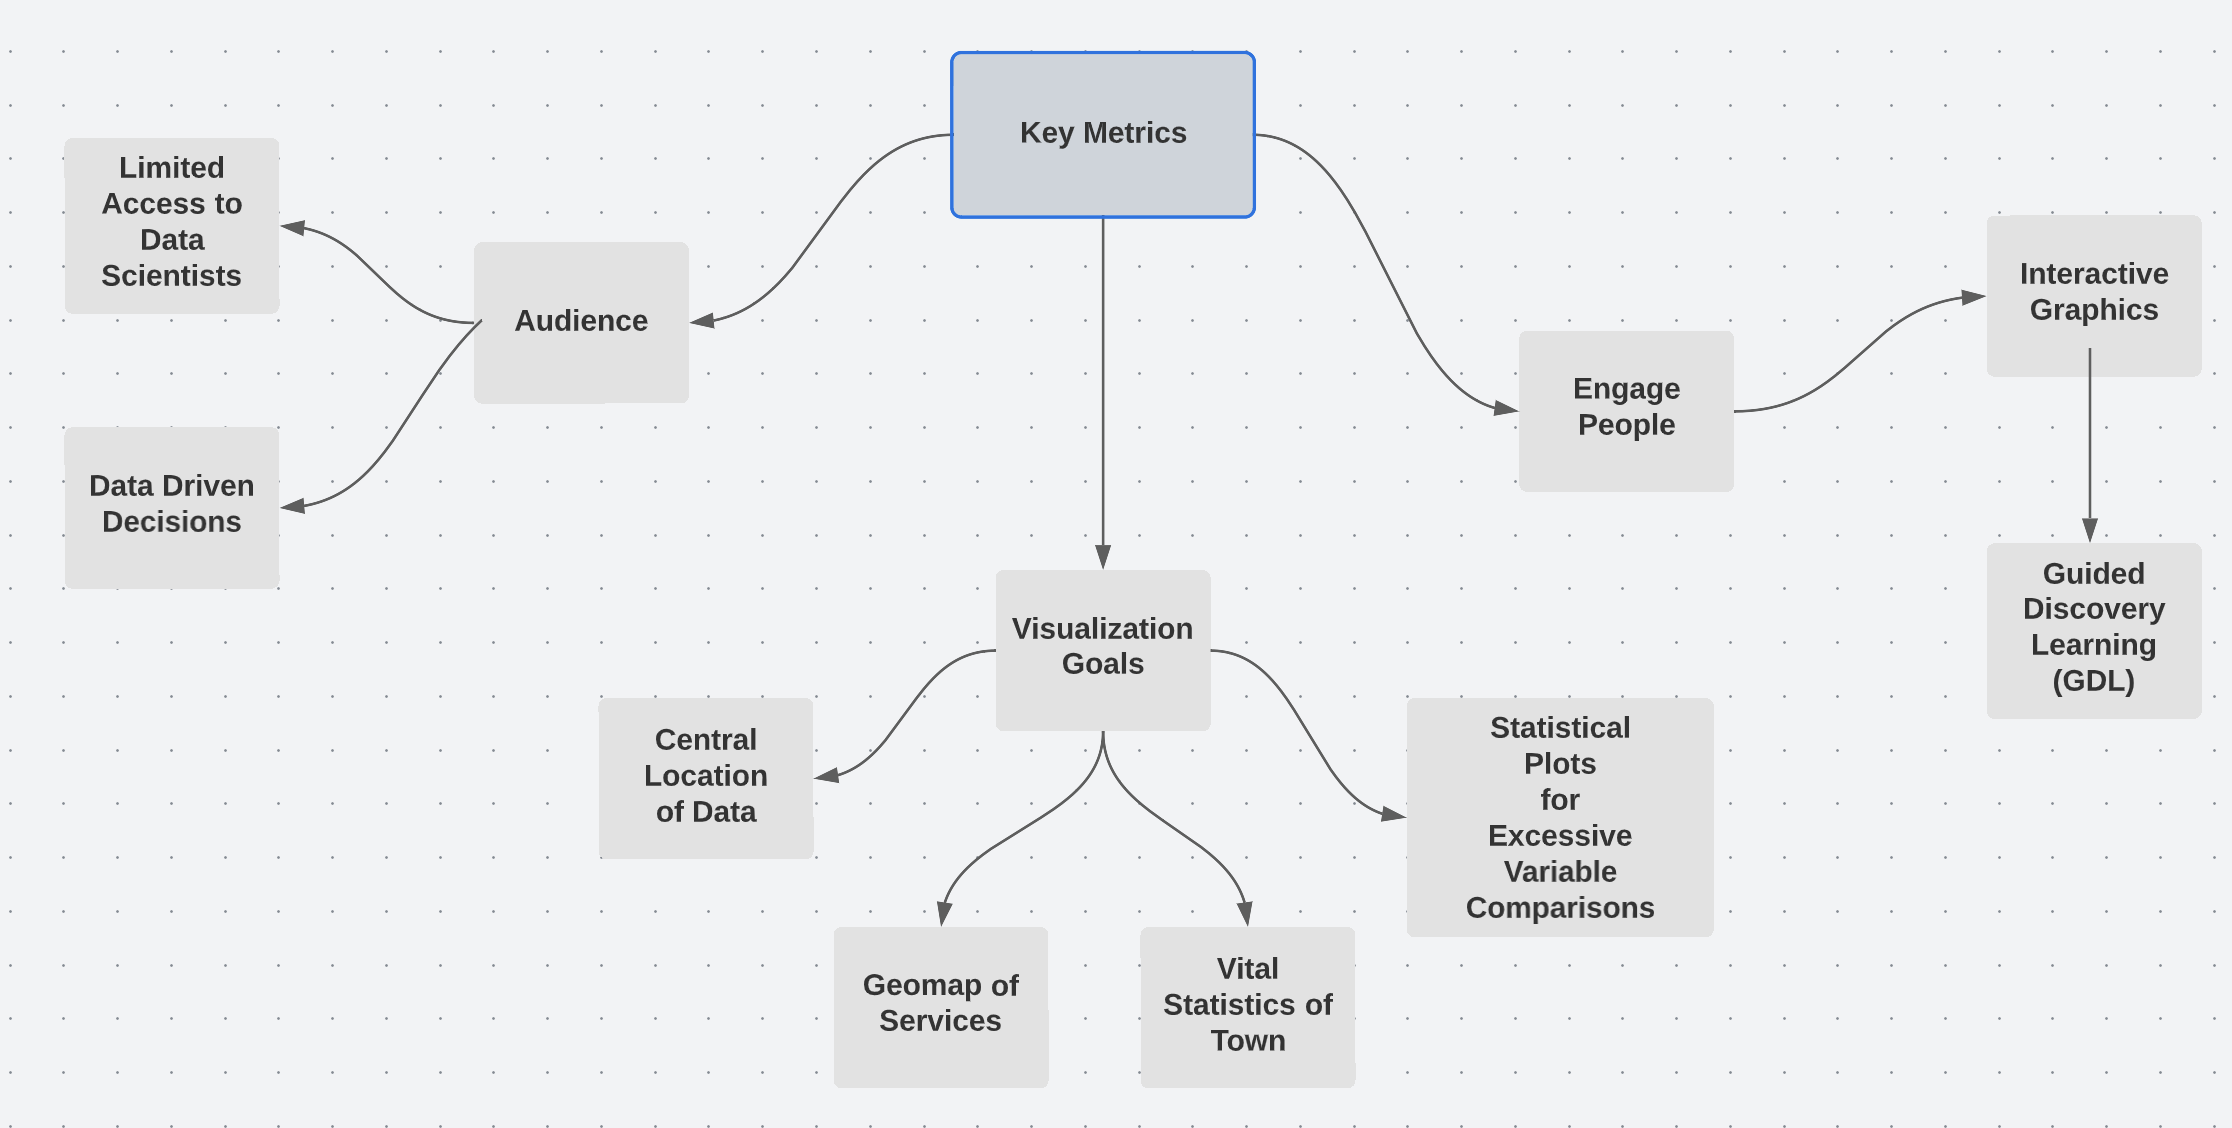
\includegraphics[width=.8\textwidth]{figure/Key_Metrics}
\caption{Diagram of considerations for our dashboard design process.}\label{fig:metrics}
\end{figure}

One problem we identified early in the process of assessing smart-shrinkage strategies in small towns is that these towns do not have the resources to make data-driven decisions. Typically, small towns in Iowa are managed by at most a few part-time employees or volunteers. In some cases, essential management functions of the town are paid, but the municipalities we are interested in do not have sufficient funding to hire professionals to gather and analyze data.

As part of a wider project investigating the strategies towns use to maintain quality of life amid shrinking population, our research team provides communities with data about their own town, but also comparable towns across the state which may have a different approach to city services. In combination with other engagement strategies that are more qualitative, we hope to use this interactive dashboard approach to assist small Iowa cities with generalizing and developing strategies to improve or maintain quality of life amid shrinking populations.

One factor at the forefront of our visualization design is the importance of reducing the cognitive demands on viewers: we have assembled an incredible amount of data, and it is easy for even statisticians who deal with much larger datasets to get lost in the details of this data. At the same time, we want to invite viewers to engage with the data - to imagine, to draw comparisons, to generalize across towns, and to integrate outside information into the conclusions drawn based on the data we present.
This invitation to engage with the data is similar to the approach advocated in Guided Discovery Learning, a framework leverages hints, feedback, and other helpful information to guide users in interactive exploration (DeDonno, 2016).

We expect that users will be interested in ``sets'' of variables from the wider dataset, which we assembled based on quality of life factors in the Iowa Small Town Poll (Peters, 2019). For instance, users might be interested in medical and social services available to residents, such as a local primary care clinic, nursing homes which are within driving distance, and the distance to the nearest emergency room; these factors might be explored separately from variables describing the services provided directly by city government, such as parks and recreation expenditures, snow removal services, and the distance to the closest fire station.

As a consequence of this massively multivariate structure, we very quickly focused on the use of parallel coordinate plots; other alternatives, such as tours (Wickham, Cook, Hofmann, \& Buja, 2011), require much more sustained attention to interactive plots as well as a deeper understanding of projections in multidimensional space which we cannot assume our users will have. Introduced in the 1880s (d'Ocagne, 1885), parallel coordinate or parallel set plots feature a series of vertical axes representing different variables arranged horizontally, with lines connecting each observation. When representing categorical data, parallel set plots may show ``blocks'' of data instead of individual lines, and are useful for representing conditional relationships between adjacent variables (Bendix, Kosara, \& Hauser, 2005); modifications of this design, such as common-angle plots (Hofmann \& Vendettuoli, 2013a), address the issues which arise due to line-width illusions VanderPlas \& Hofmann (2015). Parallel coordinate plots have been generalized to allow for continuous data and additional summaries beyond individual data points, such as densities (Heinrich \& Weiskopf, 2009). In this paper, we use the \texttt{ggpcp} package, which leverages the grammar-of-graphics framework introduced in Wickham (2016), allowing us to use not only parallel coordinate plots, but also to overlay other statistical summaries, such as boxplots or violin plots, to provide additional context about the marginal distributions of each variable in addition to allowing for exploration of the multivariate space.

We also anticipate that users will be interested in comparing their town to other, similar towns. We will discuss the different ways that this comparison strategy was implemented in each dashboard in the next section, which describes the evolution of the dashboard over time and accounting for feedback from users and other researchers on the wider project.

One final component of this project is that our dashboard is part of a wider effort to work with towns to understand the different strategies used to maintain resident quality of life amid shrinking populations. Thus, while the town leaders are our primary audience, we also are creating this applet for use in parallel with a team of other researchers: sociologists, economists, city planning specialists, and artists. These researchers opinions and feedback about the dashboard are also useful and important, as they regularly work with town leaders in different capacities and have an understanding of what factors are most important to them and what types of questions these leaders may have when faced with data and unfamiliar statistical visualizations.

Throughout the design process, we will assess our visualizations to determine which strategies for user interface and interactive graphics design are most useful to empower town leaders to make discoveries in publicly available data assembled with a focus on items that impact rural quality of life.

\hypertarget{guiding-design-principles}{%
\section{Guiding Design Principles}\label{guiding-design-principles}}

Research on dashboard creation and interactive visualization tends to be very task-specific and hard to apply to more generalized settings. That is, it is relatively easy to create a dashboard that works for a particular task, but it is hard to generalize from that process what will work for the next dashboard. With this in mind, we set out to clearly document our intentions at each stage of the design and evaluation process, with the goal of gathering some useful information about general dashboard design from the process of creating this specific dashboard.

Thus, our initial set of dashboard design principles is as follows:

\begin{itemize}
\item The town leaders are the focus audience; thus, the town itself should be the central focus of the app.
\item We should facilitate comparisons with other towns in order to allow the user to explore other potential solutions to offering services that enhance resident quality of life.
\item We will present the user with peer comparisons in order to widen the scope of exploration beyond the initial set of obvious peers in the local region.
\item We will implement feedback mechanisms that allow us to provide more detailed data and respond to feature requests to improve the dashboard design over time.
\end{itemize}

As with many dashboards, this project is under continuous development; while it makes for an unsatisfactory conclusion, we do not have a ``final'' dashboard design because the application will continue to evolve. However, we have some useful insights into the process of creating an application designed to invite users to explore a large and complex dataset that we believe to be a useful contribution to work in this area.

\hypertarget{dashboard-design-process}{%
\section{Dashboard Design Process}\label{dashboard-design-process}}

\hypertarget{dashboard-components}{%
\subsection{Dashboard Components}\label{dashboard-components}}

In this section, we discuss the philosophy behind the basic ``building blocks'' of the dashboard. This philosophy is present in all of the iterations of the dashboard that we present in this discussion, and we will evaluate the overall philosophy's effectiveness in the conclusion.

The large set of publicly available data (primarily from \url{data.iowa.gov}) we have assembled is useful, but we must be careful with how we present this data because it would be easy to overwhelm the user with small details that mask the bigger picture. We select a small subset of towns (out of the 999 towns in Iowa) and a small subset of variables of interest to start with, and then allow the user to increase the complexity of the display in accordance with their interest. This avoids some of the pitfalls of dashboard design that can easily lead to user overload (Few, 2006).

Our primary objective is to provide users with a town-centric approach: their town is at the center of our application, and comparisons to other, similar towns are secondary. As a result, the next component of the dashboard is intended to provide a brief overview of the information we have about a specific town of interest. This design is based on research into visualization sensemaking (Lee et al., 2016), in that we allow users to explore outward from the familiar to the unknown. The map visuals were built using Open Source Routing Machine (OSRM) route functions (Luxen \& Vetter, 2011) in R (R Core Team, 2022) to amplify the accuracy of the distances from necessary services in town-centric point. OSRM allows for finding the ``As the Crow Flies'' distance and time on the road for our vital services map, since OSRM technology is similar to Google maps.

When faced with the next component, a parallel coordinate plot (PCP), a novice user will be able to determine two basic components: Visual Object (textual objects and non-textual objects) and Frame (frame of content and frame of visual encoding).

Taken together, the app is a single page; the initial ``solid ground'' which the user explores from consists of maps showing the route from the center of town to necessary services, including the fire department, schools, post offices, and hospitals. In version 2, as shown in \autoref{fig:v2}, the map portion is condensed, and more space is given to value boxes that show vital statistics about the town's QoL and financial metrics. This relatively straightforward display is followed by a parallel coordinate plot that allows the user to see similar towns along dimensions such as economic indicators or population size.

\hypertarget{initial-draft}{%
\subsection{Initial Draft}\label{initial-draft}}

The initial design sketch and implementation are shown in \autoref{fig:v1}.

Users' towns are at the center of our application, and comparisons to other, similar towns are secondary. As it can be extremely difficult to predict which towns are optimal for comparison purposes (similar may involve population, region, economic indicators, sports rivalries, and any number of other variables), we allow users to modify a set of suggested comparison towns to indicate other towns of interest.

\begin{figure}
\centering
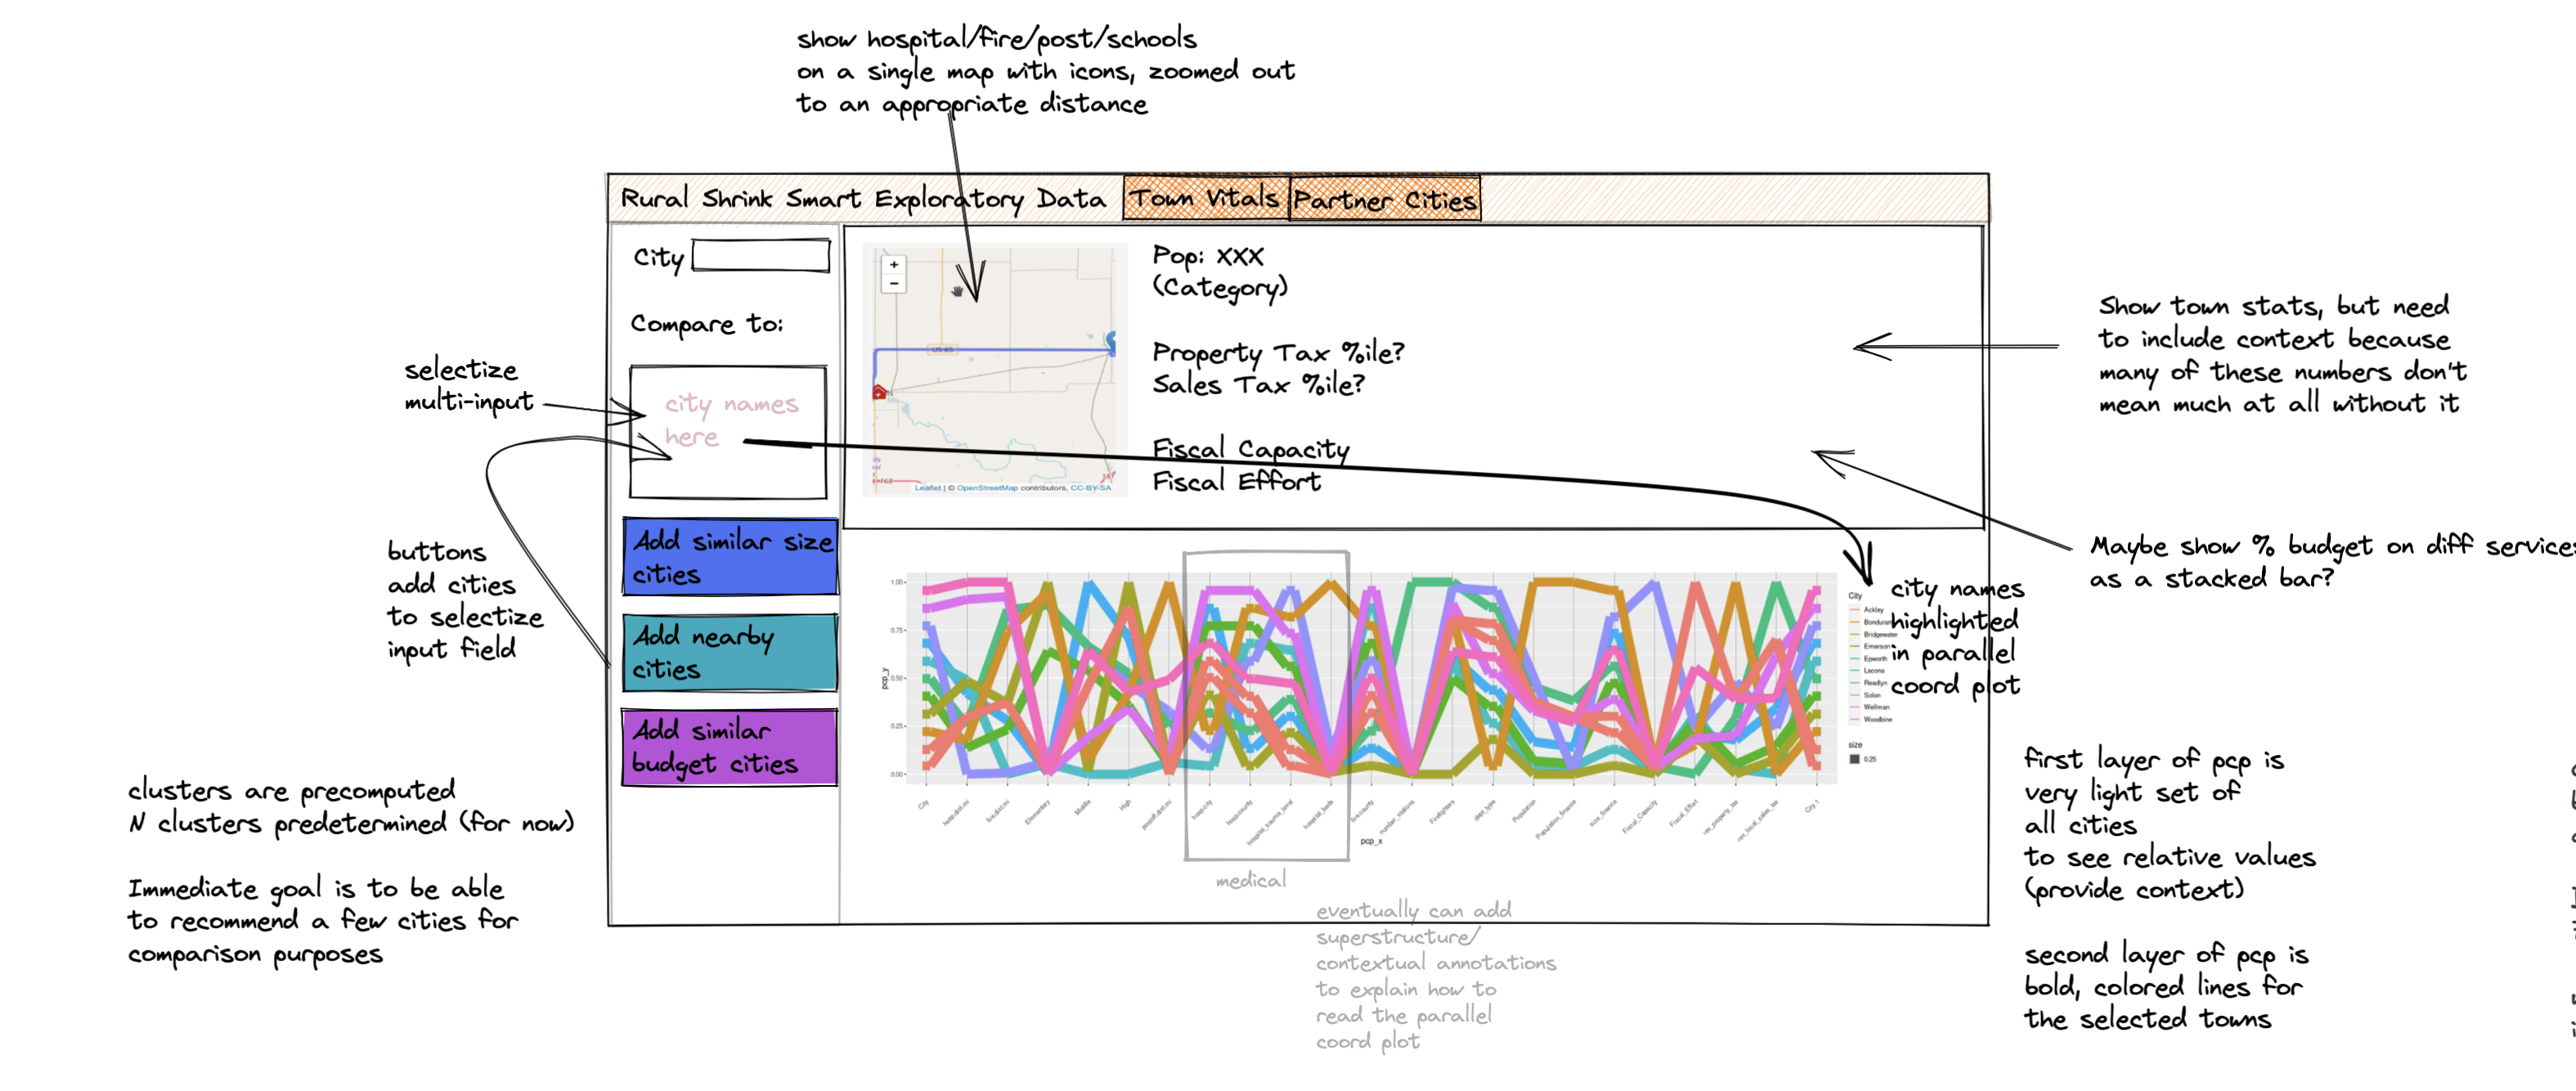
\includegraphics[width=\textwidth]{figure/Version1}

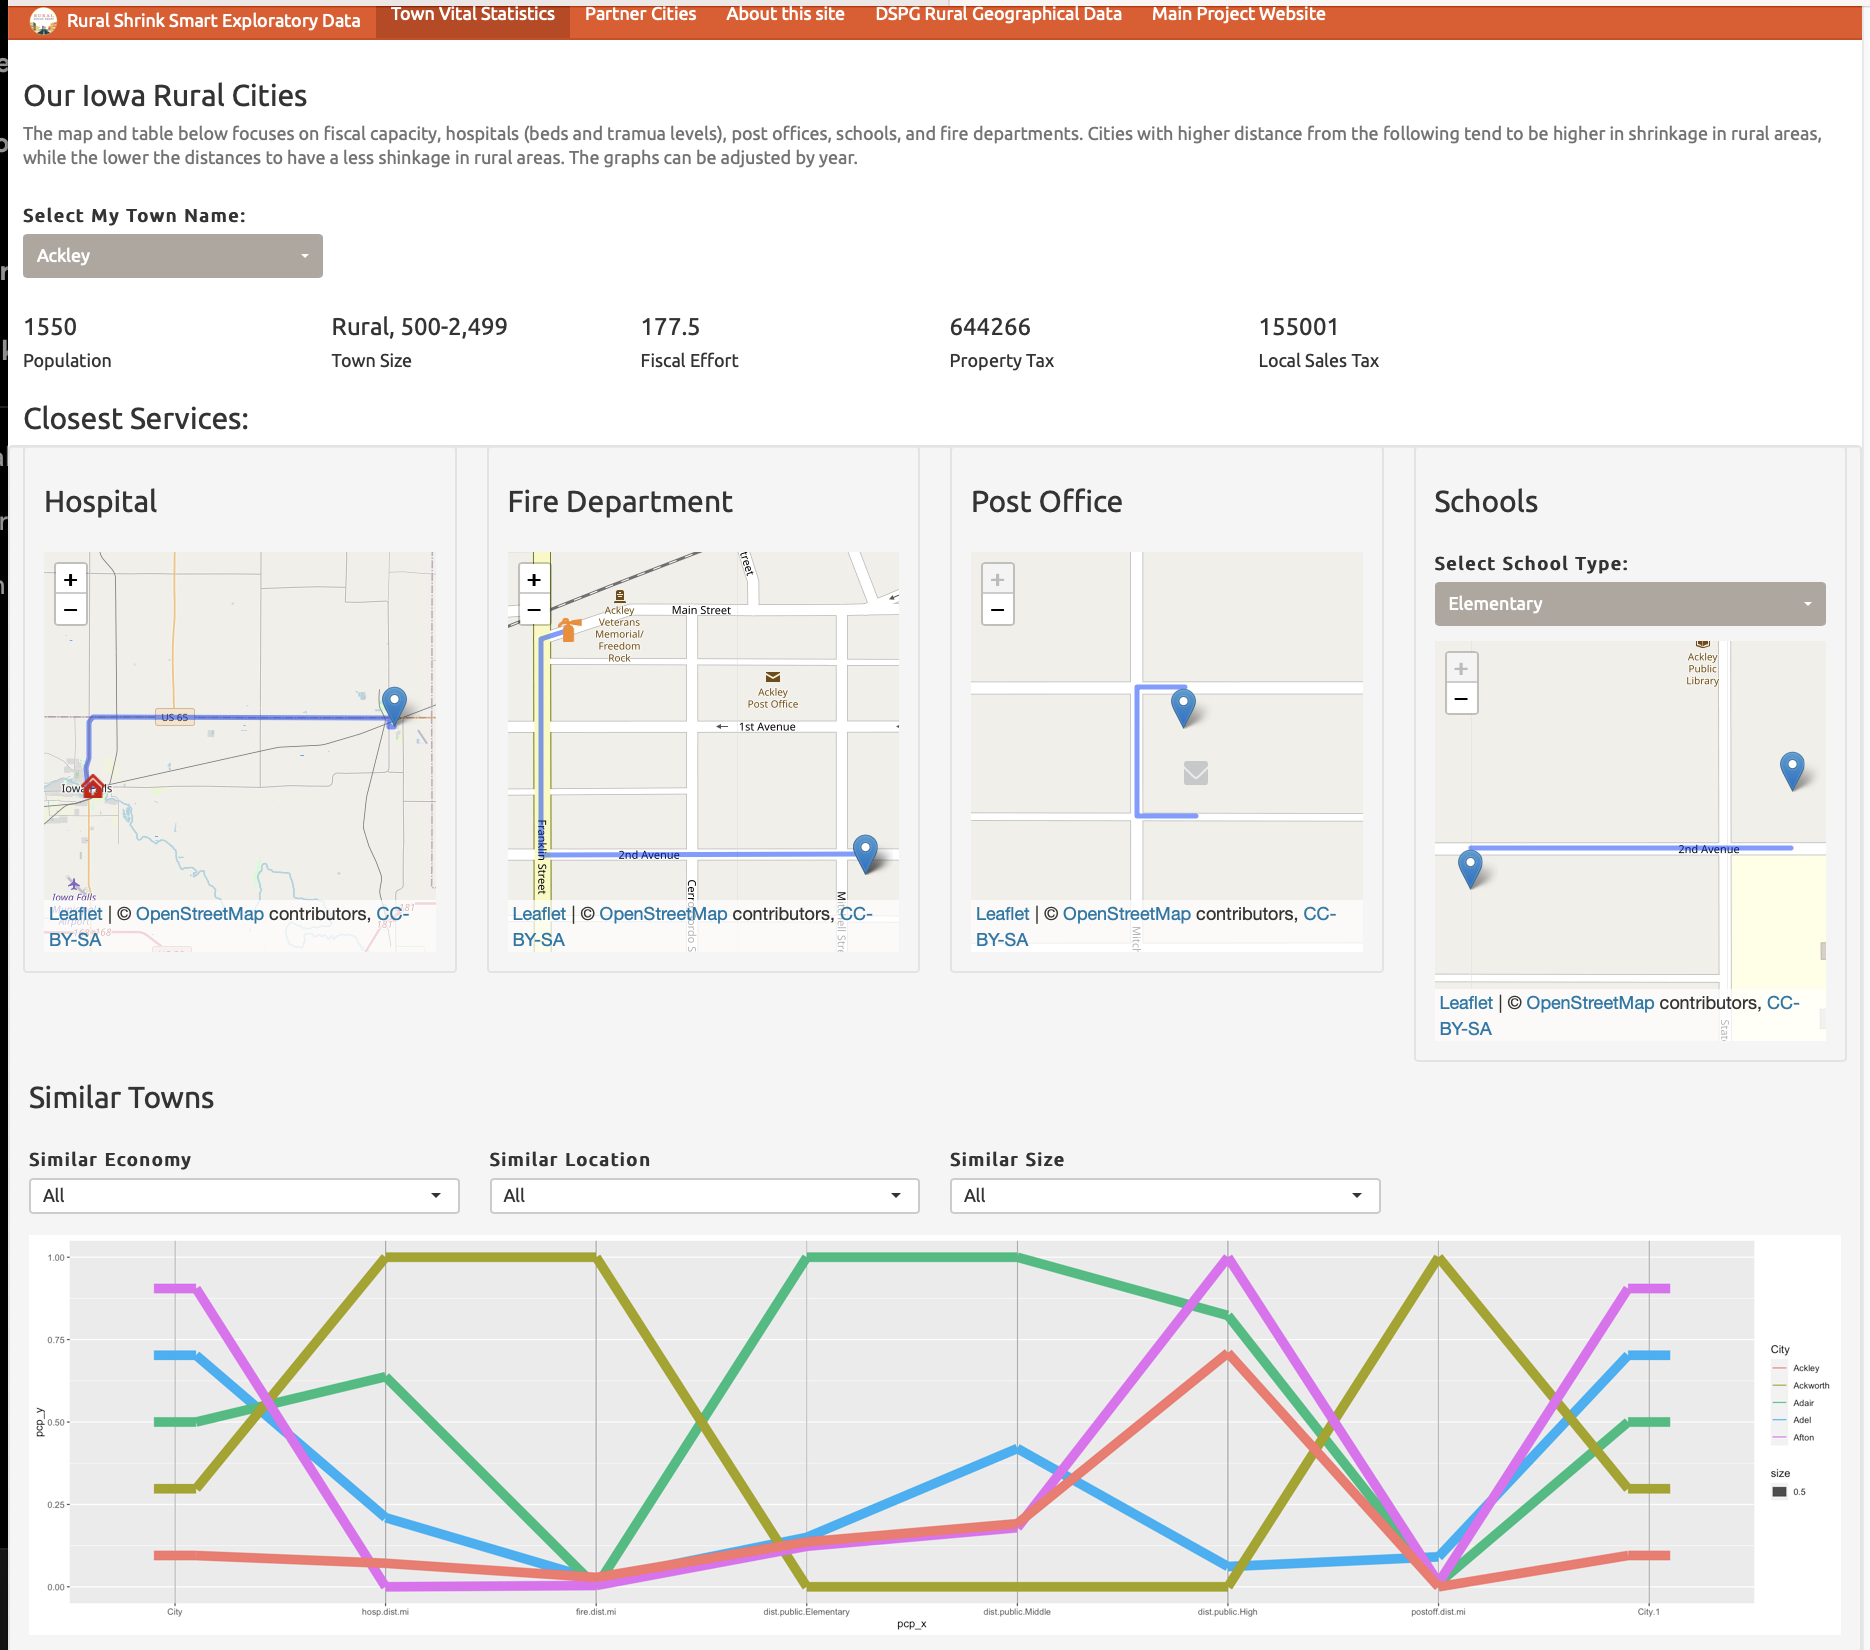
\includegraphics[width=.7\textwidth]{figure/Version2}
\caption{Initial dashboard design sketch (top) and implementation (bottom).}\label{fig:v1}
\end{figure}

We implemented some suggested town comparisons using unsupervised clustering methods to help our towns make decisions that are informed in comparison to similar towns, for budget size, population size and location. We initially focused on determining the next five to ten similar towns, based on distances to services. This feature became an important diagnostic for our data quality, as it became clear that towns which were grouped with big cities but which did not have a large population were so grouped because of missing data. Unfortunately, this clustering feature was not as useful to the application users, as they came to the dashboard with a pre-existing set of towns to compare to; our suggested comparisons were in the way.

The initial dashboard design featured several responsive maps showing the distance to the nearest hospital, fire department, post office, and school. These maps were ineffective for several reasons:

\begin{itemize}
\tightlist
\item
  Town residents already know this information (though it was useful for us as the dashboard designers, because we aren't nearly as familiar with the 900+ small towns in Iowa)
\item
  We computed distance from services relative to the center of town - coordinates provided in the data from \url{data.iowa.gov}. Generally speaking, the post office is at the center of town and the fire department is usually very close to the center of town; these two maps were useless. The school and hospital maps were less useless, but still did not provide particularly useful information to people already familiar with the town.
\item
  It became clear that it might be more useful to show the comparison towns on a map (relative to the town of interest) so that users could compare geographical ratings for unfamiliar data to familiar data.
\end{itemize}

In addition, we received feedback on the parallel coordinate plot at the bottom of the app which was surprising: the viewers (in this case, other researchers on the team) were not as intimidated by the parallel coordinate plot as we had expected. They did need some explanation of how to read the plot, and these hints need to be included in the dashboard, but they grasped the fundamental idea of the plot very quickly.

Our conclusion, based on this initial dashboard draft, was that we needed to restructure the application. Our attempt to show familiar information first to ``build up'' to the more unfamiliar structure of a parallel coordinate plot was not effective; there was too much clutter and not enough new information to draw users in.

\hypertarget{redesign}{%
\subsection{Redesign}\label{redesign}}

\begin{figure}
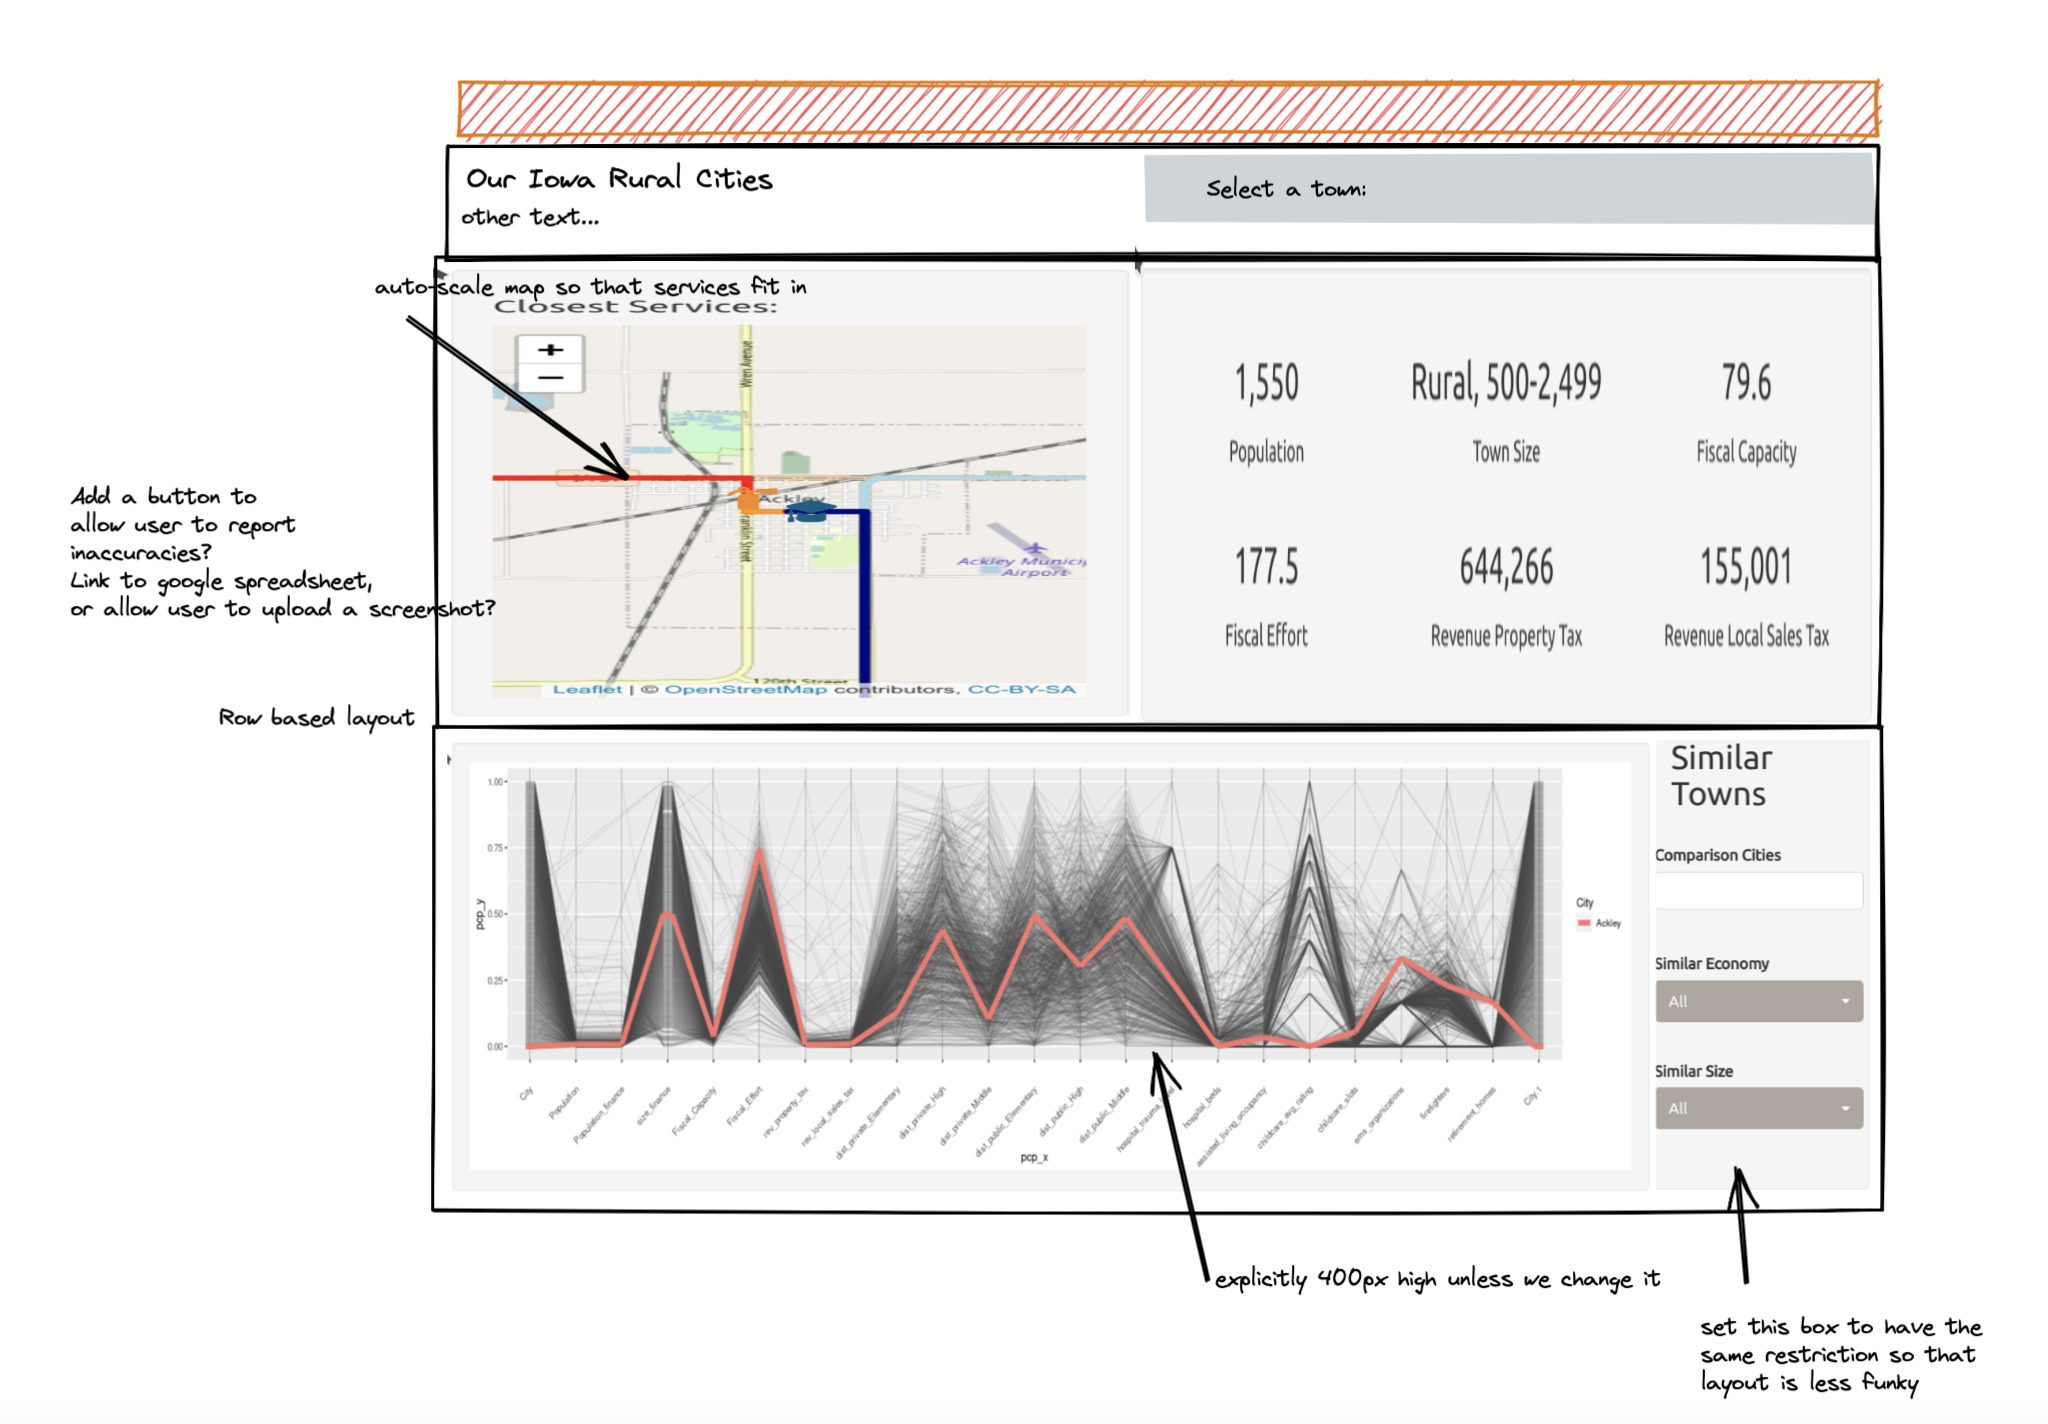
\includegraphics[width=.8\textwidth]{figure/Version3}

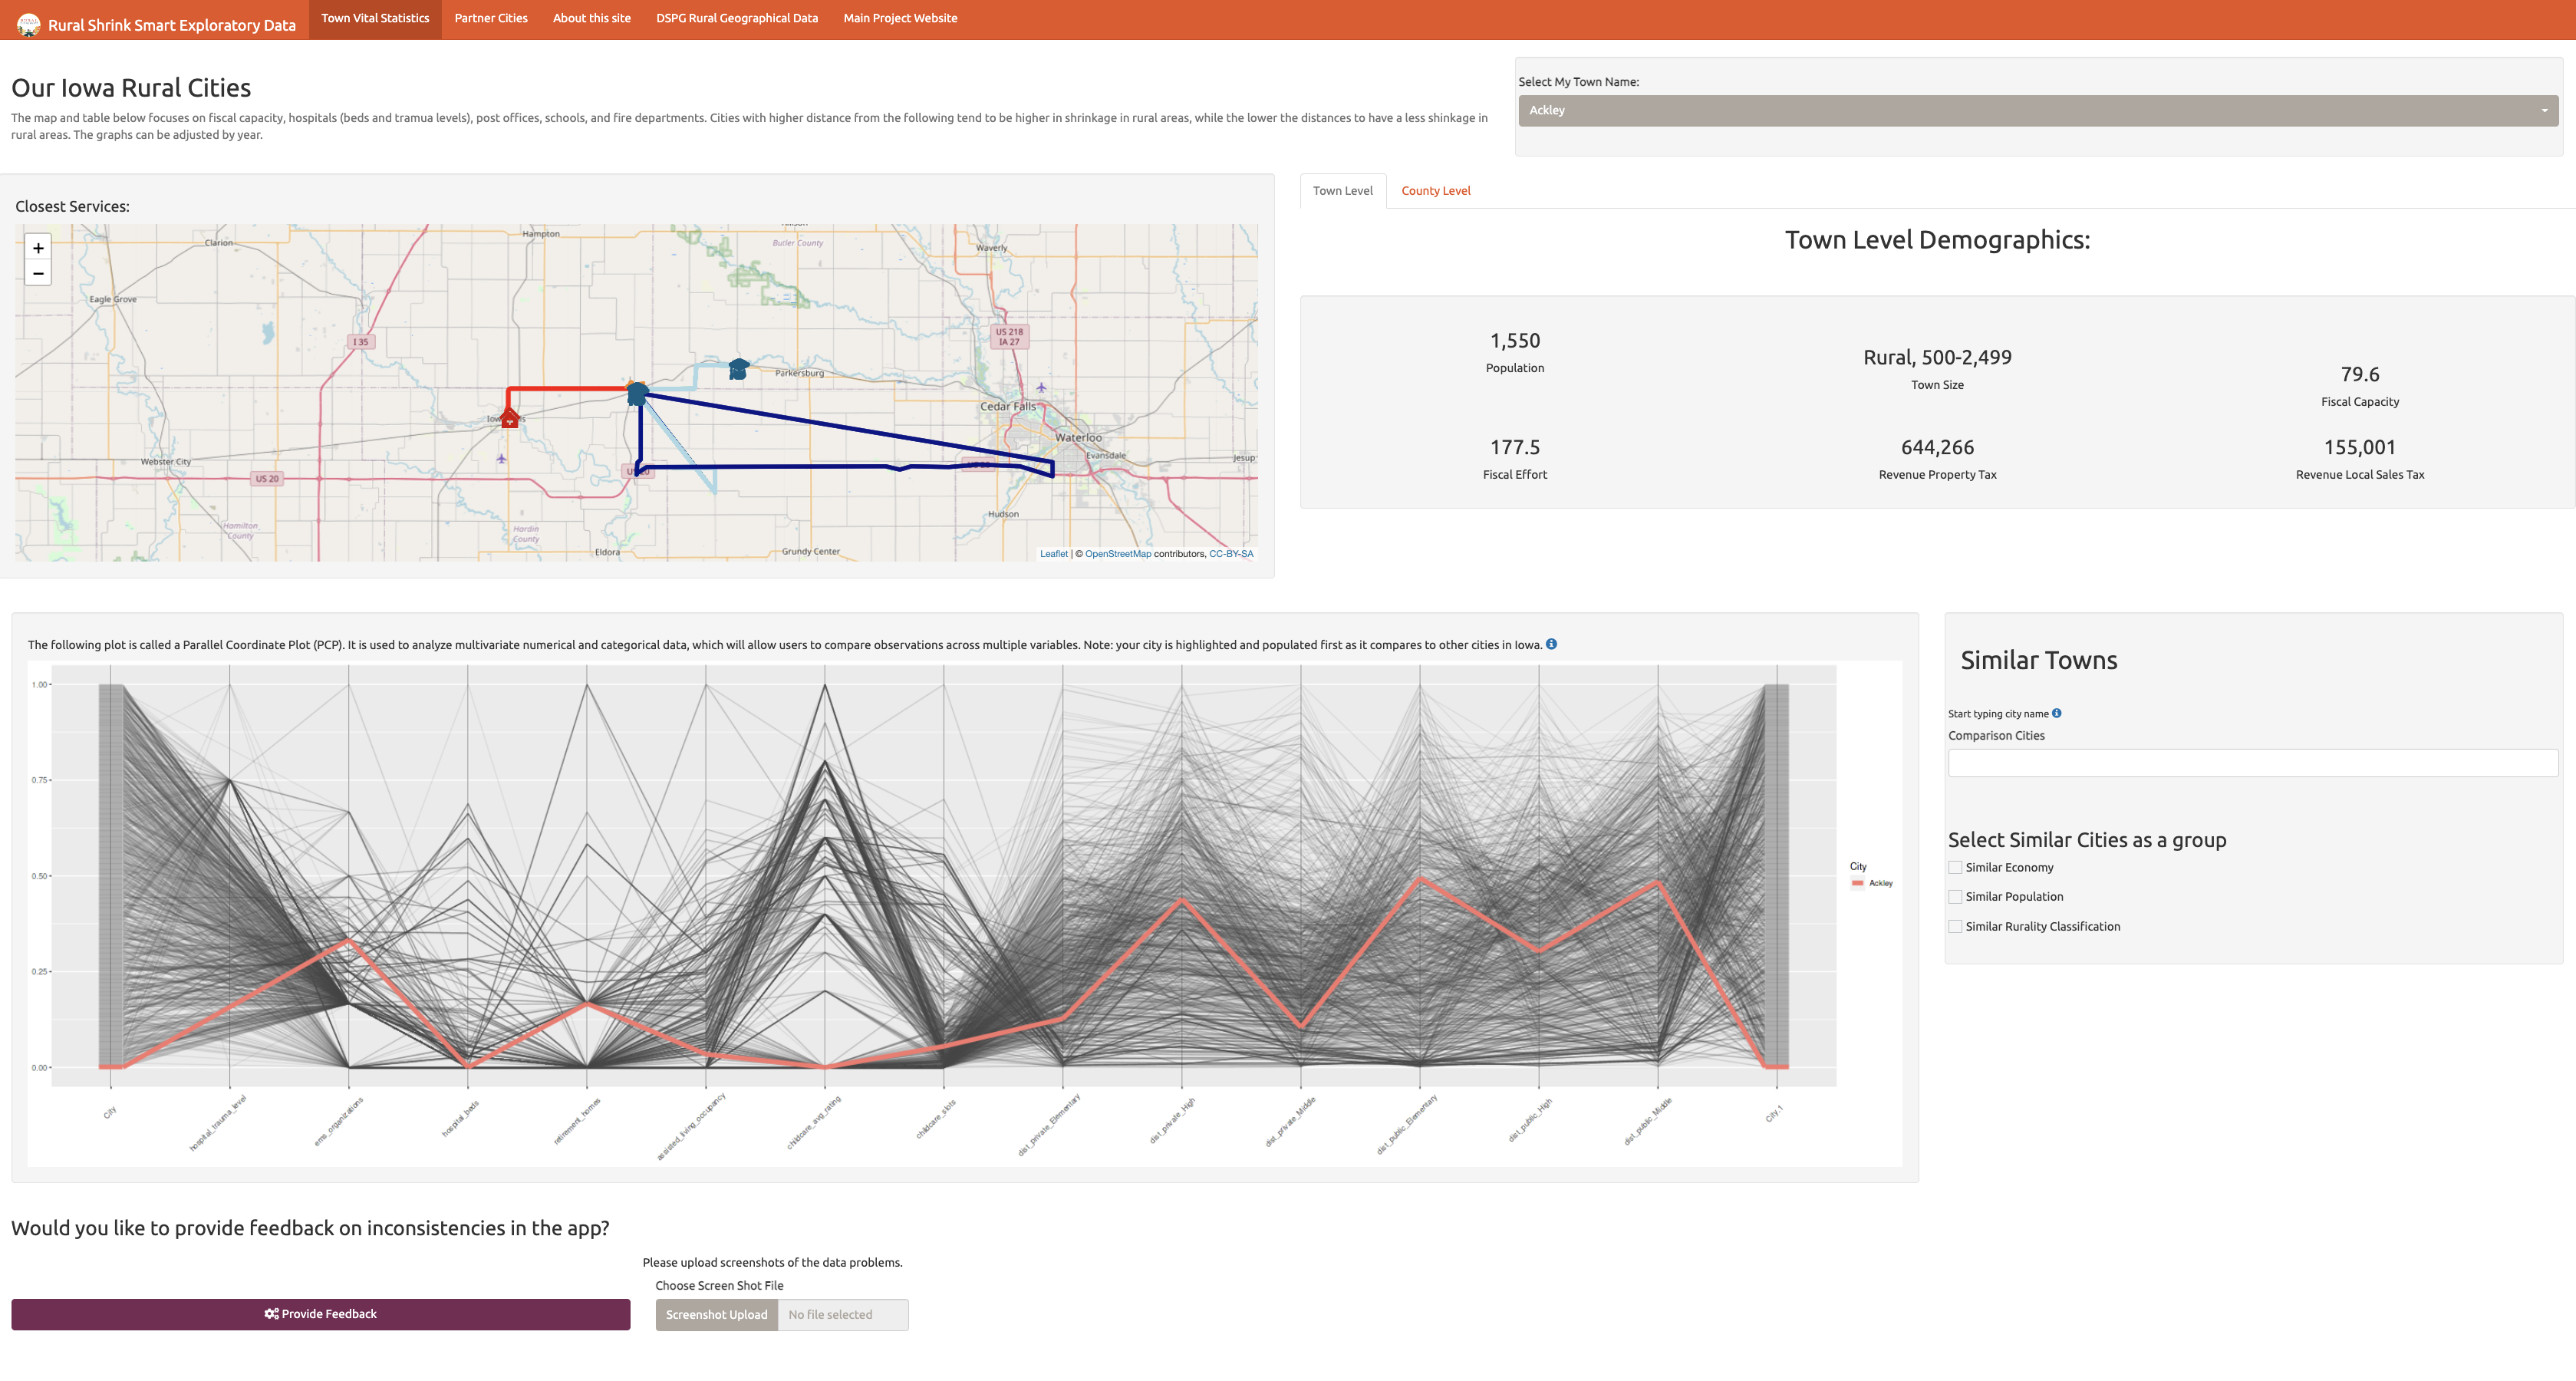
\includegraphics[width=\textwidth]{figure/Version4}
\caption{A second iteration of the sketched design (top) and the implementation (bottom).}\label{fig:v2}
\end{figure}

In the initial design, we included a map for each vital service, this initially created a lag for the users' experience. As a result, we cached map directions from OSRM for each service in our database, which drastically reduced the response time for the user. Our initial design did not naturally focus the user's eye on the most important parts of the dashboard; the redesign allowed for a cleaner flow from the top to the bottom.

In addition to the timing due to the map loading slowly, we added the vital statistics at the county level to allow for a more robust understanding of the town and it's surroundings. The rurality index provided a better classification and the USDA sources allowed for the town to understand the impact of the closest major city due to commuting for work and shopping at larger stores not available within the town.

We also modified the parallel coordinate plots in several ways:

\begin{itemize}
\tightlist
\item
  Our x-axis had a large number of variables that we as researchers believed to be the most strongly associated with quality of life. However, there were still too many variables for users to successfully parse. We reduced the number of variables, focusing on variables that had the highest data quality, and we grouped these variables by quality of life factor (Peters, 2019).
\item
  Originally, parallel coordinate bands were scaled based on the selected comparison towns. This had the effect of truncating the range of variables and over-emphasizing differences between selected towns relative to the overall range of each variable over all towns in our data set. We chose to show all towns in the data set in a very light \(\alpha\) grey color to provide some information about the overall range of each variable. Unfortunately, even with the low-\(\alpha\) value, this increased the visual complexity of the plot and confused users. Future iterations will likely make use of another aesthetic, such as boxplots or violin plots, to show the range of values for all towns, and then use lines only for towns that are selected by the user. This should strike a balance between visual complexity and representing the data accurately.
\item
  We noticed that users did not make use of our suggested comparison towns, and so we removed that option in favor of allowing users to enter their own comparison towns directly. Users already had pre-determined towns they wanted to compare to, and our suggestions were just in the way.
\end{itemize}

While not all of these modifications were well received in our second round of user testing, the changes did incrementally move the dashboard display towards our goal of allowing users to explore the data and engage with it. We continued to be surprised with how well users reacted to the parallel coordinate plots, which we initially thought might be too abstract for users unfamiliar with multivariate data displays, but the ability to compare towns across multiple dimensions and examine the similarities and differences between their approaches to different services seemed to be intuitive for users once they understood that each vertical axis was a different variable.

\hypertarget{discussion}{%
\section{Discussion}\label{discussion}}

Our dashboard design philosophy worked primarily to promote a town-centric approach application with comparisons to other similar towns being secondary. This approach created a way for the user to see their town information at the top of the page and to explore the PCP after reviewing their own town's essential statistics. The PCP in the lower part of the dashboard allowed for the user to see the plot and adjust to the fact that they could add more towns to the plot, providing an opportunity to explore the wider dataset from a base of familiar knowledge.

While we initially framed the design around guided discovery learning, the approach did not seem to suffice for our user base; instead, we found that users were more drawn to the unfamiliar from the start. We will likely leverage this in future iterations by using visual forms such as flower plots to draw the users in; even though these plots are not ideal for numerical display of data, the visual novelty and aesthetic appeal will provide some motivation to continue exploring and thinking about the data.

One factor that we have briefly considered and have seen hints of in our user feedback is that towns may not want to be compared negatively with other towns. While users have very definite ideas about which towns they would like to compare to, we can always mask the town names and move back to comparisons based on town size and other factors (for instance, whether or not a town is the county seat is a factor that is important outside of population). Using this approach, we would label each town as ``Town 1,'' ``Town 2,'' and so on, which would eliminate some of the fears about negative comparisons, but would also remove some of the novelty of the data dashboard for our users and would prevent users from drawing on their own outside knowledge about each of the comparison towns.

We also recognize that we need to leverage the expertise of others in our research team: we are working with artists, researchers in architecture, economists, and sociologists; these researchers provide outside knowledge that we do not have and may be able to help us create insightful use-cases to showcase the app and teach towns how to use it. We can also leverage the app to connect users with our research team, providing additional value to those who use the applet and facilitating development of strategies for maintaining quality of life amid shrinking populations.

\hypertarget{future-work}{%
\section{Future Work}\label{future-work}}

One avenue we will explore in future iterations of the dashboard is to incorporate other dashboards generated by different groups within this project. This will create a wider field of information to explore: for instance, some of the additional work will focus on the 99 towns featured in the Iowa Small Town Poll; this will allow us to showcase survey-based measures of quality of life alongside the more objective measurements assembled in the dataset discussed in this paper. While at least one tab of this omni-dashboard will still focus on wider EDA and discovery, we hope to incorporate other information as well to provide a more well-rounded data display encompassing most of the facets of this complex project.

We are also mindful of a distinction between ``eye candy'' and purpose-driven data visualization. While we have typically focused on the latter, there is certainly a place in our dashboard for the former as well. ``Eye candy'' visualization is intended to draw the viewer in and motivate them to explore; while these visualizations may not be particularly effective at communicating quantitative information, if they motivate the user to engage with the rest of the dashboard, they still serve a purpose. It is with this mindset that we intend to explore the use of flower plots - the artistic opportunities combined with the display of quantitative information (even in a form that isn't optimal for quantitative comparisons) may be useful to engage viewers before transitioning to more useful data visualizations intended to provide accurate quantitative comparisons.

EDA can be a difficult for a variety of groups of people, novice users and experienced researchers. One of the more difficult components of this project has been clearly articulating the purposes of EDA to a diverse group of researchers unfamiliar with the concept. One of the most useful parts of this dashboard iteration process has been as an aid to data discovery: that is, the dashboard motivated us to find additional data sources and incorporate them into the project. Having conversations with other researchers about the EDA process helped to facilitate these conversations, as each discussion seemed to uncover additional data sources that someone remembered after looking at the dashboard. While this facet of the dashboard process may be difficult to study formally, it would be an interesting avenue for investigation.

\hypertarget{conclusions}{%
\section{Conclusions}\label{conclusions}}

In this paper, we have documented the process of designing a dashboard for exploration and visualization of a large and complex data set assembled from many different sources. Our primary audience was leaders of small towns in Iowa, with a secondary audience of researchers in fields other than statistics collaborating on this project with us. Through the process of revising our dashboard, we found that the idea of guided discovery learning as implemented in our first version did not work as well as we had anticipated. It was more important to focus on allowing users to explore their questions about the dataset by facilitating user-driven comparisons and exploration, rather than attempting to anticipate user desires by providing comparison towns. In addition, we found that it would be more effective to draw users in with novel visual displays, as these seemed to attract more interest than providing known facts and an opportunity to explore outwards from an initial area of familiarity.

While it is hard to apply the findings from one fairly specific visualization project more widely, there is a lack of resources in this area that provide both design philosophies and actual analysis of user feedback in a qualitative sense. We have attempted to address this dearth of information by providing the design strategies, user feedback, and our planned and executed modifications, in the hopes that others facing the daunting challenge of designing a dashboard for EDA may learn something from our experiences.

\hypertarget{math-sci}{%
\chapter{Chapter 2 Stuff}\label{math-sci}}

\hypertarget{ref-labels}{%
\chapter{Tables, Graphics, References, and Labels}\label{ref-labels}}

\hypertarget{tables}{%
\section{Tables}\label{tables}}

By far the easiest way to present tables in your thesis is to store the contents of the table in a CSV or Excel file, then read that file in to your R Markdown document as a data frame. Then you can style the table with the \texttt{kable} function, or functions in the \href{https://cran.r-project.org/web/packages/kableExtra/index.html}{kableExtra} pacakge.

In addition to the tables that can be automatically generated from a data frame in \textbf{R} that you saw in {[}R Markdown Basics{]} using the \texttt{kable} function, you can also create tables using \emph{pandoc}. (More information is available at \url{http://pandoc.org/README.html\#tables}.) This might be useful if you don't have values specifically stored in \textbf{R}, but you'd like to display them in table form. Below is an example. Pay careful attention to the alignment in the table and hyphens to create the rows and columns. Generally I don't recommend this approach of typing the table directly into your R Markdown document.

\begin{longtable}[]{@{}
  >{\centering\arraybackslash}p{(\columnwidth - 4\tabcolsep) * \real{0.31}}
  >{\centering\arraybackslash}p{(\columnwidth - 4\tabcolsep) * \real{0.51}}
  >{\centering\arraybackslash}p{(\columnwidth - 4\tabcolsep) * \real{0.18}}@{}}
\caption{\label{tab:inher} Correlation of Inheritance Factors for Parents and Child}\tabularnewline
\toprule
Factors & Correlation between Parents \& Child & Inherited \\
\midrule
\endfirsthead
\toprule
Factors & Correlation between Parents \& Child & Inherited \\
\midrule
\endhead
Education & -0.49 & Yes \\
Socio-Economic Status & 0.28 & Slight \\
Income & 0.08 & No \\
Family Size & 0.18 & Slight \\
Occupational Prestige & 0.21 & Slight \\
\bottomrule
\end{longtable}

We can also create a link to the table by doing the following: Table \ref{tab:inher}. If you go back to {[}Loading and exploring data{]} and look at the \texttt{kable} table, we can create a reference to this max delays table too: Table \ref{tab:maxdelays}. The addition of the \texttt{(\textbackslash{}\#tab:inher)} option to the end of the table caption allows us to then make a reference to Table \texttt{\textbackslash{}@ref(tab:label)}. Note that this reference could appear anywhere throughout the document after the table has appeared.

\clearpage

\hypertarget{figures}{%
\section{Figures}\label{figures}}

If your thesis has a lot of figures, \emph{R Markdown} might behave better for you than that other word processor. One perk is that it will automatically number the figures accordingly in each chapter. You'll also be able to create a label for each figure, add a caption, and then reference the figure in a way similar to what we saw with tables earlier. If you label your figures, you can move the figures around and \emph{R Markdown} will automatically adjust the numbering for you. No need for you to remember! So that you don't have to get too far into LaTeX to do this, a couple \textbf{R} functions have been created for you to assist. You'll see their use below.

In the \textbf{R} chunk below, we will load in a picture stored as \texttt{uw.png} in our main directory. We then give it the caption of ``UW logo,'' the label of ``uwlogo,'' and specify that this is a figure. Make note of the different \textbf{R} chunk options that are given in the R Markdown file (not shown in the knitted document).

\begin{Shaded}
\begin{Highlighting}[]
\FunctionTok{include\_graphics}\NormalTok{(}\AttributeTok{path =} \StringTok{"figure/unl.png"}\NormalTok{)}
\end{Highlighting}
\end{Shaded}

\begin{figure}

\includegraphics[width=\linewidth]{figure/unl} \caption{logo}\label{fig:uwlogo}
\end{figure}

Here is a reference to the UW logo: Figure \ref{fig:uwlogo}. Note the use of the \texttt{fig:} code here. By naming the \textbf{R} chunk that contains the figure, we can then reference that figure later as done in the first sentence here. We can also specify the caption for the figure via the R chunk option \texttt{fig.cap}.

\clearpage

Below we will investigate how to save the output of an \textbf{R} plot and label it in a way similar to that done above. Recall the \texttt{flights} dataset from Chapter \ref{rmd-basics}. (Note that we've shown a different way to reference a section or chapter here.) We will next explore a bar graph with the mean flight departure delays by airline from Portland for 2014. Note also the use of the \texttt{scale} parameter which is discussed on the next page.

\begin{Shaded}
\begin{Highlighting}[]
\NormalTok{flights }\SpecialCharTok{\%\textgreater{}\%}
    \FunctionTok{group\_by}\NormalTok{(carrier) }\SpecialCharTok{\%\textgreater{}\%}
    \FunctionTok{summarize}\NormalTok{(}\AttributeTok{mean\_dep\_delay =} \FunctionTok{mean}\NormalTok{(dep\_delay)) }\SpecialCharTok{\%\textgreater{}\%}
    \FunctionTok{ggplot}\NormalTok{(}\FunctionTok{aes}\NormalTok{(}\AttributeTok{x =}\NormalTok{ carrier, }\AttributeTok{y =}\NormalTok{ mean\_dep\_delay)) }\SpecialCharTok{+}
    \FunctionTok{geom\_bar}\NormalTok{(}\AttributeTok{position =} \StringTok{"identity"}\NormalTok{, }\AttributeTok{stat =} \StringTok{"identity"}\NormalTok{,}
        \AttributeTok{fill =} \StringTok{"red"}\NormalTok{)}
\end{Highlighting}
\end{Shaded}

\begin{figure}
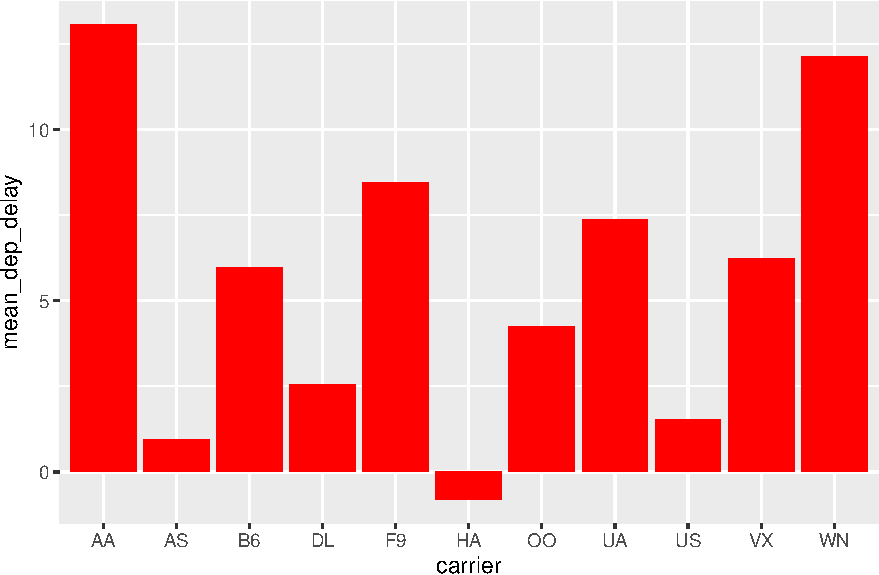
\includegraphics[width=\linewidth]{thesis_files/figure-latex/delaysboxplot-1} \caption{Mean Delays by Airline}\label{fig:delaysboxplot}
\end{figure}

Here is a reference to this image: Figure \ref{fig:delaysboxplot}.

A table linking these carrier codes to airline names is available at \url{https://github.com/ismayc/pnwflights14/blob/master/data/airlines.csv}.

\clearpage

Next, we will explore the use of the \texttt{out.extra} chunk option, which can be used to shrink or expand an image loaded from a file by specifying \texttt{"scale=\ "}. Here we use the mathematical graph stored in the ``subdivision.pdf'' file.

\begin{figure}
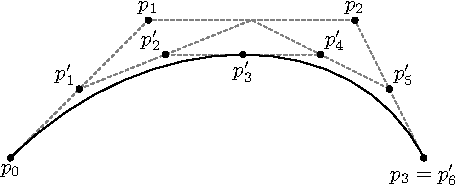
\includegraphics[width=\linewidth,scale=0.75]{figure/subdivision} \caption{Subdiv. graph}\label{fig:subd}
\end{figure}

Here is a reference to this image: Figure \ref{fig:subd}. Note that \texttt{echo=FALSE} is specified so that the \textbf{R} code is hidden in the document.

\textbf{More Figure Stuff}

Lastly, we will explore how to rotate and enlarge figures using the \texttt{out.extra} chunk option. (Currently this only works in the PDF version of the book.)

\begin{figure}
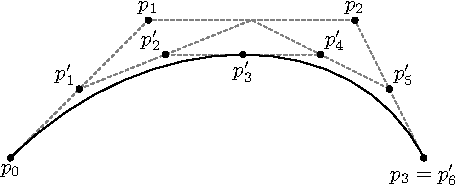
\includegraphics[width=\linewidth,angle=180, scale=1.1]{figure/subdivision} \caption{A Larger Figure, Flipped Upside Down}\label{fig:subd2}
\end{figure}

As another example, here is a reference: Figure \ref{fig:subd2}.

\hypertarget{footnotes-and-endnotes}{%
\section{Footnotes and Endnotes}\label{footnotes-and-endnotes}}

You might want to footnote something.\footnote{footnote text} The footnote will be in a smaller font and placed appropriately. Endnotes work in much the same way.

\hypertarget{cross-referencing-chapters-and-sections}{%
\section{Cross-referencing chapters and sections}\label{cross-referencing-chapters-and-sections}}

The \href{https://bookdown.org/yihui/bookdown/cross-references.html}{bookdown documentation} is an excellent source for learning how to cross-reference in a bookdown project such as a huskydown document. Here we only cover the most common uses for a typical thesis. If you want something more complex or fancy, please refer to the bookdown documentation and seek help from the developers of that package.

By default, all of your chapter and section headers will get an auto-generated ID label For example, e.g., \texttt{\#\ Chapter\ 1} will have an auto-generated ID \texttt{chapter-1}. Note that the ID label is all lower case, and has no spaces. If you have any kind of punctuation in your header, such as a colon (:), it will not appear in the ID label. Then in your text you can reference chapter one in your Rmd file like this: `as discussed in Chapter \texttt{\textbackslash{}@ref(chapter-1)},' which will print as `as discussed in Chapter 1'

We strongly recommend that you to manually assign ID labels to your chapter header to make it easy to cross-reference. For example, at the top of the Rmd file for this chapter, you can see:

\texttt{\#\ Tables,\ Graphics,\ References,\ and\ Labels\ \{\#ref-labels\}}

The \texttt{\{\#ref-labels\}} part of this header is the ID label. It doesn't show in the output, but is there for us to use for easy cross-referencing, because it can be short, and we don't need to change it elsewhere our document when we update the chapter header. We can use this custom ID label in our Rmd document like this: `as discussed in Chapter \texttt{\textbackslash{}@ref(ref-labels)},' which will print as `as discussed in Chapter \ref{ref-labels}.' If you need to show custom text instead of the chapter number, you use this syntax in your Rmd document: \texttt{see\ {[}my\ chapter\ about\ labels{]}(\#ref-labels)\ for\ more\ details} which will appear as `see \protect\hyperlink{ref-labels}{my chapter about labels} for more details'

To cross-reference a specific section in the same chapter, we recommend adding a custom ID label to the section header, and using that to cross-reference. For example, earlier in this chapter we have a section on tables and in the Rmd file we see \texttt{\#\#\ Tables\ \{\#tables\}}. We can cross-reference that in the text like this `as discussed in the section on \texttt{{[}tables{]}(\#tables)}' which will appear as `as discussed in the above section on \protect\hyperlink{tables}{tables}'

To cross-reference a section in a different chapter we can use the ID label from that section directly. For example, we can write in our Rmd document \texttt{as\ discussed\ in\ the\ section\ on\ {[}R\ code\ chunks{]}(\#r-chunks)\ in\ Chapter\ \textbackslash{}@ref(rmd-basics)} which will appear as `as discussed in the section on \protect\hyperlink{r-chunks}{R code chunks} in Chapter \ref{rmd-basics}.'

If you prefer to cross-reference by the section number, we can use custom ID labels in our Rmd document. For example, to refer to a section in our first chapter, we can write in the Rmd document: \texttt{as\ discussed\ in\ section\ \textbackslash{}@ref(r-chunks)\ in\ Chapter\ \textbackslash{}@ref(rmd-basics)}. This will appear with section and chapter numbers like so: as `as discussed in section \ref{r-chunks} in Chapter \ref{rmd-basics}.'

\hypertarget{bibliographies}{%
\section{Bibliographies}\label{bibliographies}}

Of course you will need to cite things, and you will probably accumulate an armful of sources. There are a variety of tools available for creating a bibliography database (stored with the .bib extension). In addition to BibTeX suggested below, you may want to consider using the free and easy-to-use tool called Zotero. Some Zotero documentation is at \url{http://libguides.reed.edu/citation/zotero}. In addition, a tutorial is available from Middlebury College at \url{http://sites.middlebury.edu/zoteromiddlebury/}.

\emph{R Markdown} uses \emph{pandoc} (\url{http://pandoc.org/}) to build its bibliographies. One nice caveat of this is that you won't have to do a second compile to load in references as standard LaTeX requires. To cite references in your thesis (after creating your bibliography database), place the reference name inside square brackets and precede it by the ``at'' symbol. For example, here's a reference to a book about worrying: (Molina \& Borkovec, 1994). This \texttt{Molina1994} entry appears in a file called \texttt{thesis.bib} in the \texttt{bib} folder. This bibliography database file was created by a program called BibTeX. You can call this file something else if you like (look at the YAML header in the main .Rmd file) and, by default, is to placed in the \texttt{bib} folder.

For more information about BibTeX and bibliographies, see (\url{http://web.reed.edu/cis/help/latex/index.html})\footnote{Reed~College (2007)}. There are three pages on this topic: \emph{bibtex} (which talks about using BibTeX, at \url{http://web.reed.edu/cis/help/latex/bibtex.html}), \emph{bibtexstyles} (about how to find and use the bibliography style that best suits your needs, at \url{http://web.reed.edu/cis/help/latex/bibtexstyles.html}) and \emph{bibman} (which covers how to make and maintain a bibliography by hand, without BibTeX, at \url{http://web.reed.edu/cis/help/latex/bibman.html}). The last page will not be useful unless you have only a few sources.

If you look at the YAML header at the top of the main .Rmd file you can see that we can specify the style of the bibliography by referencing the appropriate csl file. You can download a variety of different style files at \url{https://www.zotero.org/styles}. Make sure to download the file into the csl folder.

\textbf{Tips for Bibliographies}

\begin{itemize}
\tightlist
\item
  Like with thesis formatting, the sooner you start compiling your bibliography for something as large as thesis, the better.
\item
  The cite key (a citation's label) needs to be unique from the other entries.
\item
  When you have more than one author or editor, you need to separate each author's name by the word ``and'' e.g.~\texttt{Author\ =\ \{Noble,\ Sam\ and\ Youngberg,\ Jessica\},}.
\item
  Bibliographies made using BibTeX (whether manually or using a manager) accept LaTeX markup, so you can italicize and add symbols as necessary.
\item
  To force capitalization in an article title or where all lowercase is generally used, bracket the capital letter in curly braces.
\end{itemize}

\hypertarget{anything-else}{%
\section{Anything else?}\label{anything-else}}

If you'd like to see examples of other things in this template, please \href{https://github.com/benmarwick/huskydown/issues/new}{contact us} (email \href{mailto:bmarwick@uw.edu}{\nolinkurl{bmarwick@uw.edu}}) with your suggestions. We love to see people using \emph{R Markdown} for their theses, and are happy to help.

\hypertarget{conclusion-1}{%
\chapter*{Conclusion}\label{conclusion-1}}
\addcontentsline{toc}{chapter}{Conclusion}

If we don't want Conclusion to have a chapter number next to it, we can add the \texttt{\{-\}} attribute.

\textbf{More info}

And here's some other random info: the first paragraph after a chapter title or section head \emph{shouldn't be} indented, because indents are to tell the reader that you're starting a new paragraph. Since that's obvious after a chapter or section title, proper typesetting doesn't add an indent there.

\appendix

\hypertarget{the-first-appendix}{%
\chapter{The First Appendix}\label{the-first-appendix}}

This first appendix includes all of the R chunks of code that were hidden throughout the document (using the \texttt{include\ =\ FALSE} chunk tag) to help with readibility and/or setup.

\textbf{In the main Rmd file}

\begin{Shaded}
\begin{Highlighting}[]
\CommentTok{\# This chunk ensures that the huskydown}
\CommentTok{\# package is installed and loaded. This}
\CommentTok{\# huskydown package includes the template}
\CommentTok{\# files for the thesis.}
\ControlFlowTok{if}\NormalTok{ (}\SpecialCharTok{!}\FunctionTok{require}\NormalTok{(devtools)) }\FunctionTok{install.packages}\NormalTok{(}\StringTok{"devtools"}\NormalTok{,}
    \AttributeTok{repos =} \StringTok{"http://cran.rstudio.com"}\NormalTok{)}
\CommentTok{\# if(!require(huskydown))}
\CommentTok{\# devtools::install\_github(}
\CommentTok{\# \textquotesingle{}benmarwick/huskydown\textquotesingle{} )}
\CommentTok{\# library(huskydown)}
\FunctionTok{library}\NormalTok{(knitr)}
\FunctionTok{library}\NormalTok{(palmerpenguins)}
\FunctionTok{library}\NormalTok{(tidyverse)}
\end{Highlighting}
\end{Shaded}

\textbf{In Chapter \ref{ref-labels}:}

\begin{Shaded}
\begin{Highlighting}[]
\CommentTok{\# This chunk ensures that the huskydown}
\CommentTok{\# package is installed and loaded. This}
\CommentTok{\# huskydown package includes the template}
\CommentTok{\# files for the thesis and also two}
\CommentTok{\# functions used for labeling and}
\CommentTok{\# referencing}
\ControlFlowTok{if}\NormalTok{ (}\SpecialCharTok{!}\FunctionTok{require}\NormalTok{(devtools)) }\FunctionTok{install.packages}\NormalTok{(}\StringTok{"devtools"}\NormalTok{,}
    \AttributeTok{repos =} \StringTok{"http://cran.rstudio.com"}\NormalTok{)}
\ControlFlowTok{if}\NormalTok{ (}\SpecialCharTok{!}\FunctionTok{require}\NormalTok{(dplyr)) }\FunctionTok{install.packages}\NormalTok{(}\StringTok{"dplyr"}\NormalTok{,}
    \AttributeTok{repos =} \StringTok{"http://cran.rstudio.com"}\NormalTok{)}
\ControlFlowTok{if}\NormalTok{ (}\SpecialCharTok{!}\FunctionTok{require}\NormalTok{(ggplot2)) }\FunctionTok{install.packages}\NormalTok{(}\StringTok{"ggplot2"}\NormalTok{,}
    \AttributeTok{repos =} \StringTok{"http://cran.rstudio.com"}\NormalTok{)}
\ControlFlowTok{if}\NormalTok{ (}\SpecialCharTok{!}\FunctionTok{require}\NormalTok{(ggplot2)) }\FunctionTok{install.packages}\NormalTok{(}\StringTok{"bookdown"}\NormalTok{,}
    \AttributeTok{repos =} \StringTok{"http://cran.rstudio.com"}\NormalTok{)}
\ControlFlowTok{if}\NormalTok{ (}\SpecialCharTok{!}\FunctionTok{require}\NormalTok{(huskydown)) \{}
    \FunctionTok{library}\NormalTok{(devtools)}
\NormalTok{    devtools}\SpecialCharTok{::}\FunctionTok{install\_github}\NormalTok{(}\StringTok{"benmarwick/huskydown"}\NormalTok{)}
\NormalTok{\}}
\FunctionTok{library}\NormalTok{(huskydown)}
\NormalTok{flights }\OtherTok{\textless{}{-}} \FunctionTok{read.csv}\NormalTok{(}\StringTok{"data/flights.csv"}\NormalTok{)}
\end{Highlighting}
\end{Shaded}

\hypertarget{the-second-appendix-for-fun}{%
\chapter{The Second Appendix, for Fun}\label{the-second-appendix-for-fun}}

\hypertarget{colophon}{%
\chapter*{Colophon}\label{colophon}}
\addcontentsline{toc}{chapter}{Colophon}

This document is set in \href{https://github.com/georgd/EB-Garamond}{EB Garamond}, \href{https://github.com/adobe-fonts/source-code-pro/}{Source Code Pro} and \href{http://www.latofonts.com/lato-free-fonts/}{Lato}. The body text is set at 11pt with \(\familydefault\).

It was written in R Markdown and \(\LaTeX\), and rendered into PDF using \href{https://github.com/benmarwick/huskydown}{huskydown} and \href{https://github.com/rstudio/bookdown}{bookdown}.

This document was typeset using the XeTeX typesetting system, and the \href{http://staff.washington.edu/fox/tex/}{University of Washington Thesis class} class created by Jim Fox. Under the hood, the \href{https://github.com/UWIT-IAM/UWThesis}{University of Washington Thesis LaTeX template} is used to ensure that documents conform precisely to submission standards. Other elements of the document formatting source code have been taken from the \href{https://github.com/stevenpollack/ucbthesis}{Latex, Knitr, and RMarkdown templates for UC Berkeley's graduate thesis}, and \href{https://github.com/suchow/Dissertate}{Dissertate: a LaTeX dissertation template to support the production and typesetting of a PhD dissertation at Harvard, Princeton, and NYU}

The source files for this thesis, along with all the data files, have been organised into an R package, xxx, which is available at \url{https://github.com/xxx/xxx}. A hard copy of the thesis can be found in the University of Washington library.

This version of the thesis was generated on 2022-11-21 13:10:38. The repository is currently at this commit:

The computational environment that was used to generate this version is as follows:

\begin{verbatim}
## - Session info -------------------------------------------
##  setting  value
##  version  R version 4.1.0 (2021-05-18)
##  os       macOS Big Sur 10.16
##  system   x86_64, darwin17.0
##  ui       X11
##  language (EN)
##  collate  en_US.UTF-8
##  ctype    en_US.UTF-8
##  tz       America/New_York
##  date     2022-11-21
##  pandoc   2.11.4 @ /Applications/RStudio.app/Contents/MacOS/pandoc/ (via rmarkdown)
## 
## - Packages -----------------------------------------------
##  package        * version date (UTC) lib source
##  assertthat       0.2.1   2019-03-21 [2] CRAN (R 4.1.0)
##  backports        1.4.1   2021-12-13 [1] CRAN (R 4.1.0)
##  bookdown         0.29.1  2022-09-18 [1] Github (rstudio/bookdown@4890be2)
##  broom            0.8.0   2022-04-13 [2] CRAN (R 4.1.2)
##  cachem           1.0.6   2021-08-19 [1] CRAN (R 4.1.0)
##  callr            3.7.0   2021-04-20 [2] CRAN (R 4.1.0)
##  cellranger       1.1.0   2016-07-27 [2] CRAN (R 4.1.0)
##  cli              3.3.0   2022-04-25 [1] CRAN (R 4.1.2)
##  colorspace       2.0-3   2022-02-21 [1] CRAN (R 4.1.2)
##  crayon           1.5.1   2022-03-26 [1] CRAN (R 4.1.0)
##  DBI              1.1.2   2021-12-20 [1] CRAN (R 4.1.0)
##  dbplyr           2.1.1   2021-04-06 [2] CRAN (R 4.1.0)
##  devtools       * 2.4.4   2022-07-20 [1] CRAN (R 4.1.2)
##  digest           0.6.29  2021-12-01 [1] CRAN (R 4.1.0)
##  dplyr          * 1.0.9   2022-04-28 [1] CRAN (R 4.1.2)
##  ellipsis         0.3.2   2021-04-29 [2] CRAN (R 4.1.0)
##  evaluate         0.16    2022-08-09 [1] CRAN (R 4.1.2)
##  fansi            1.0.3   2022-03-24 [1] CRAN (R 4.1.2)
##  farver           2.1.1   2022-07-06 [1] CRAN (R 4.1.2)
##  fastmap          1.1.0   2021-01-25 [2] CRAN (R 4.1.0)
##  forcats        * 0.5.1   2021-01-27 [1] CRAN (R 4.1.0)
##  formatR          1.12    2022-03-31 [1] CRAN (R 4.1.2)
##  fs               1.5.2   2021-12-08 [1] CRAN (R 4.1.0)
##  generics         0.1.3   2022-07-05 [1] CRAN (R 4.1.2)
##  ggplot2        * 3.3.6   2022-05-03 [2] CRAN (R 4.1.2)
##  git2r            0.30.1  2022-03-16 [1] CRAN (R 4.1.2)
##  glue             1.6.2   2022-02-24 [1] CRAN (R 4.1.2)
##  gtable           0.3.0   2019-03-25 [2] CRAN (R 4.1.0)
##  haven            2.5.0   2022-04-15 [2] CRAN (R 4.1.2)
##  hms              1.1.1   2021-09-26 [1] CRAN (R 4.1.0)
##  htmltools        0.5.3   2022-07-18 [1] CRAN (R 4.1.2)
##  htmlwidgets      1.5.4   2021-09-08 [1] CRAN (R 4.1.0)
##  httpuv           1.6.5   2022-01-05 [1] CRAN (R 4.1.2)
##  httr             1.4.3   2022-05-04 [1] CRAN (R 4.1.2)
##  huskydown      * 0.0.5   2022-01-16 [1] Github (benmarwick/huskydown@addb48e)
##  jsonlite         1.8.0   2022-02-22 [1] CRAN (R 4.1.2)
##  knitr          * 1.40    2022-08-24 [1] CRAN (R 4.1.2)
##  labeling         0.4.2   2020-10-20 [2] CRAN (R 4.1.0)
##  later            1.3.0   2021-08-18 [1] CRAN (R 4.1.0)
##  lifecycle        1.0.1   2021-09-24 [1] CRAN (R 4.1.0)
##  lubridate        1.8.0   2021-10-07 [1] CRAN (R 4.1.0)
##  magrittr         2.0.3   2022-03-30 [1] CRAN (R 4.1.2)
##  memoise          2.0.1   2021-11-26 [1] CRAN (R 4.1.0)
##  mime             0.12    2021-09-28 [1] CRAN (R 4.1.0)
##  miniUI           0.1.1.1 2018-05-18 [1] CRAN (R 4.1.0)
##  modelr           0.1.8   2020-05-19 [2] CRAN (R 4.1.0)
##  munsell          0.5.0   2018-06-12 [2] CRAN (R 4.1.0)
##  palmerpenguins * 0.1.0   2020-07-23 [1] CRAN (R 4.1.0)
##  pillar           1.7.0   2022-02-01 [1] CRAN (R 4.1.2)
##  pkgbuild         1.3.1   2021-12-20 [1] CRAN (R 4.1.0)
##  pkgconfig        2.0.3   2019-09-22 [2] CRAN (R 4.1.0)
##  pkgload          1.3.0   2022-06-27 [1] CRAN (R 4.1.2)
##  prettyunits      1.1.1   2020-01-24 [2] CRAN (R 4.1.0)
##  processx         3.5.3   2022-03-25 [2] CRAN (R 4.1.2)
##  profvis          0.3.7   2020-11-02 [1] CRAN (R 4.1.0)
##  promises         1.2.0.1 2021-02-11 [1] CRAN (R 4.1.0)
##  ps               1.7.0   2022-04-23 [2] CRAN (R 4.1.2)
##  purrr          * 0.3.4   2020-04-17 [2] CRAN (R 4.1.0)
##  R6               2.5.1   2021-08-19 [1] CRAN (R 4.1.0)
##  Rcpp             1.0.9   2022-07-08 [1] CRAN (R 4.1.2)
##  readr          * 2.1.2   2022-01-30 [1] CRAN (R 4.1.2)
##  readxl           1.4.0   2022-03-28 [2] CRAN (R 4.1.2)
##  remotes          2.4.2   2021-11-30 [1] CRAN (R 4.1.0)
##  reprex           2.0.1   2021-08-05 [2] CRAN (R 4.1.0)
##  rlang            1.0.5   2022-08-31 [1] CRAN (R 4.1.2)
##  rmarkdown        2.16    2022-08-24 [1] CRAN (R 4.1.2)
##  rstudioapi       0.13    2020-11-12 [2] CRAN (R 4.1.0)
##  rvest            1.0.2   2021-10-16 [1] CRAN (R 4.1.0)
##  scales           1.2.0   2022-04-13 [2] CRAN (R 4.1.2)
##  sessioninfo      1.2.2   2021-12-06 [1] CRAN (R 4.1.0)
##  shiny            1.7.1   2021-10-02 [1] CRAN (R 4.1.0)
##  stringi          1.7.8   2022-07-11 [1] CRAN (R 4.1.0)
##  stringr        * 1.4.1   2022-08-20 [1] CRAN (R 4.1.2)
##  tibble         * 3.1.7   2022-05-03 [1] CRAN (R 4.1.2)
##  tidyr          * 1.2.0   2022-02-01 [1] CRAN (R 4.1.2)
##  tidyselect       1.1.2   2022-02-21 [1] CRAN (R 4.1.0)
##  tidyverse      * 1.3.1   2021-04-15 [2] CRAN (R 4.1.0)
##  tzdb             0.3.0   2022-03-28 [1] CRAN (R 4.1.0)
##  urlchecker       1.0.1   2021-11-30 [1] CRAN (R 4.1.0)
##  usethis        * 2.1.6   2022-05-25 [1] CRAN (R 4.1.2)
##  utf8             1.2.2   2021-07-24 [2] CRAN (R 4.1.0)
##  vctrs            0.4.1   2022-04-13 [1] CRAN (R 4.1.2)
##  withr            2.5.0   2022-03-03 [1] CRAN (R 4.1.2)
##  xfun             0.33    2022-09-12 [1] CRAN (R 4.1.2)
##  xml2             1.3.3   2021-11-30 [1] CRAN (R 4.1.0)
##  xtable           1.8-4   2019-04-21 [2] CRAN (R 4.1.0)
##  yaml             2.3.5   2022-02-21 [1] CRAN (R 4.1.2)
## 
##  [1] /Users/dbradford4/Library/R/x86_64/4.1/library
##  [2] /Library/Frameworks/R.framework/Versions/4.1/Resources/library
## 
## ----------------------------------------------------------
\end{verbatim}

\backmatter

\hypertarget{references}{%
\chapter*{References}\label{references}}
\addcontentsline{toc}{chapter}{References}

\noindent

\setlength{\parindent}{-0.20in}
\setlength{\leftskip}{0.20in}
\setlength{\parskip}{8pt}

\hypertarget{refs}{}
\begin{CSLReferences}{1}{0}
\leavevmode\hypertarget{ref-abello2002}{}%
Abello, J., \& Korn, J. (2002). MGV: A system for visualizing massive multidigraphs. \emph{IEEE Transactions on Visualization and Computer Graphics}, \emph{8}(1), 21--38. http://doi.org/\href{https://doi.org/10.1109/2945.981849}{10.1109/2945.981849}

\leavevmode\hypertarget{ref-angel2000}{}%
Angel, E. (2000). \emph{Interactive computer graphics : A top-down approach with OpenGL}. Boston, MA: Addison Wesley Longman.

\leavevmode\hypertarget{ref-angel2001}{}%
Angel, E. (2001a). \emph{Batch-file computer graphics : A bottom-up approach with QuickTime}. Boston, MA: Wesley Addison Longman.

\leavevmode\hypertarget{ref-angel2002a}{}%
Angel, E. (2001b). \emph{Test second book by angel}. Boston, MA: Wesley Addison Longman.

\leavevmode\hypertarget{ref-bartlett1932}{}%
Bartlett, F. A., \& Remembering, A. (1932). A study in experimental and social psychology. New York: Cambridge University Press.

\leavevmode\hypertarget{ref-Bendix:2005}{}%
Bendix, F., Kosara, R., \& Hauser, H. (2005). {Parallel Sets: Visual Analysis of Categorical Data}. In \emph{2005 IEEE symposium on information visualization (INFOVIS'05)} (pp. 133--140). IEEE. http://doi.org/\href{https://doi.org/10.1109/INFOVIS.2005.27}{10.1109/INFOVIS.2005.27}

\leavevmode\hypertarget{ref-booth2006}{}%
Booth, J. L., \& Siegler, R. S. (2006). Developmental and individual differences in pure numerical estimation. \emph{Developmental Psychology}, \emph{42}(1), 189.

\leavevmode\hypertarget{ref-brunswik1952}{}%
Brunswik, E. (1952). \emph{The conceptual framework of psychology} (Vol. 1). University of Chicago Press.

\leavevmode\hypertarget{ref-buja2009}{}%
Buja, A., Cook, D., Hofmann, H., Lawrence, M., Lee, E.-K., Swayne, D. F., \& Wickham, H. (2009). Statistical inference for exploratory data analysis and model diagnostics. \emph{Philosophical Transactions of the Royal Society A: Mathematical, Physical and Engineering Sciences}, \emph{367}(1906), 4361--4383.

\leavevmode\hypertarget{ref-card1999}{}%
Card, S. K., Mackinlay, J. D., \& Shneiderman, B. (1999). Using vision to think. \emph{Readings in Information Visualization: Using Vision to Think}, 579--581.

\leavevmode\hypertarget{ref-carley1992}{}%
Carley, K., \& Palmquist, M. (1992). Extracting, representing, and analyzing mental models. \emph{Social Forces}, \emph{70}(3), 601--636.

\leavevmode\hypertarget{ref-choo2009}{}%
Choo, C. W. (2009). Information use and early warning effectiveness: Perspectives and prospects. \emph{Journal of the American Society for Information Science and Technology}, \emph{60}(5), 1071--1082.

\leavevmode\hypertarget{ref-cowan2001}{}%
Cowan, N. (2001). The magical number 4 in short-term memory: A reconsideration of mental storage capacity. \emph{Behavioral and Brain Sciences}, \emph{24}(1), 87--114.

\leavevmode\hypertarget{ref-dOcagne:1885}{}%
d'Ocagne, M. (1885). {Coordonnées parallèles et axiales : Méthode de transformation géométrique et procédé nouveau de calcul graphique déduits de la considération des coordonnées parallèles}. \emph{Gauthier-Villars}, 112. Retrieved from \url{https://archive.org/details/coordonnesparal00ocaggoog/page/n10}

\leavevmode\hypertarget{ref-sine}{}%
Day, R. H., \& Stecher, E. J. (1991). Sine of an illusion. \emph{Perception}, \emph{20}, 49--55.

\leavevmode\hypertarget{ref-dedonno}{}%
DeDonno, M. A. (2016). The influence of IQ on pure discovery and guided discovery learning of a complex real-world task. \emph{Learning and Individual Differences}, \emph{49}, 11--16.

\leavevmode\hypertarget{ref-JHPHDashboard}{}%
Dong E, G. L., Du H. (2022). An interactive web-based dashboard to track COVID-19 in real time. http://doi.org/\href{https://doi.org/10.1016/S1473-3099(20)30120-1}{10.1016/S1473-3099(20)30120-1}

\leavevmode\hypertarget{ref-few}{}%
Few, S. (2006). \emph{Information dashboard design: The effective visual communication of data}. Newton, MA: O'Reilly Media, Inc.

\leavevmode\hypertarget{ref-friedman1979}{}%
Friedman, A. (1979). Framing pictures: The role of knowledge in automatized encoding and memory for gist. \emph{Journal of Experimental Psychology: General}, \emph{108}(3), 316.

\leavevmode\hypertarget{ref-heaps1999}{}%
Heaps, C., \& Handel, S. (1999). Similarity and features of natural textures. \emph{Journal of Experimental Psychology: Human Perception and Performance}, \emph{25}(2), 299.

\leavevmode\hypertarget{ref-density-pcp}{}%
Heinrich, J., \& Weiskopf, D. (2009). {Continuous Parallel Coordinates}. \emph{IEEE Transactions on Visualization and Computer Graphics}, \emph{15}(6), 1531--1538. http://doi.org/\href{https://doi.org/10.1109/TVCG.2009.131}{10.1109/TVCG.2009.131}

\leavevmode\hypertarget{ref-heylighen1997}{}%
Heylighen, F. (1997). Publications on complex, evolving systems: A citation-based survey. \emph{Complexity}, \emph{2}(5), 31--36.

\leavevmode\hypertarget{ref-ggpcp}{}%
Hofmann, H., VanderPlas, S., \& Ge, Y. (2022). \emph{Ggpcp: Parallel coordinate plots in the ggplot2 framework}. Retrieved from \url{https://github.com/heike/ggpcp}

\leavevmode\hypertarget{ref-Heike2013}{}%
Hofmann, H., \& Vendettuoli, M. (2013b). Common angle plots as perception-true visualizations of categorical associations. \emph{IEEE Transactions on Visualization and Computer Graphics}, \emph{19}(12), 2297--2305. http://doi.org/\href{https://doi.org/10.1109/TVCG.2013.140}{10.1109/TVCG.2013.140}

\leavevmode\hypertarget{ref-Hofmann:2013}{}%
Hofmann, H., \& Vendettuoli, M. (2013a). {Common Angle Plots as Perception-True Visualizations of Categorical Associations}. \emph{IEEE Transactions on Visualization and Computer Graphics}, \emph{19}(12), 2297--2305. http://doi.org/\href{https://doi.org/10.1109/TVCG.2013.140}{10.1109/TVCG.2013.140}

\leavevmode\hypertarget{ref-huang2006}{}%
Huang, Z., Chen, H., Guo, F., Xu, J. J., Wu, S., \& Chen, W.-H. (2006). Expertise visualization: An implementation and study based on cognitive fit theory. \emph{Decision Support Systems}, \emph{42}(3), 1539--1557.

\leavevmode\hypertarget{ref-Hurley}{}%
Hurley, C. (2019). \emph{Gclus: Clustering graphics}. Retrieved from \url{https://CRAN.R-project.org/package=gclus}

\leavevmode\hypertarget{ref-Inselberg}{}%
Inselberg, A. (1985). {The plane with parallel coordinates}. \emph{The Visual Computer}, \emph{1}(2), 69--91. http://doi.org/\href{https://doi.org/10.1007/BF01898350}{10.1007/BF01898350}

\leavevmode\hypertarget{ref-kiem2002}{}%
Keim, D. A. (2002). Information visualization and visual data mining. \emph{IEEE Transactions on Visualization and Computer Graphics}, \emph{8}(1), 1--8. http://doi.org/\href{https://doi.org/10.1109/2945.981847}{10.1109/2945.981847}

\leavevmode\hypertarget{ref-klein2007}{}%
Klein, G., Phillips, J. K., Rall, E. L., \& Peluso, D. A. (2007). A data--frame theory of sensemaking. In \emph{Expertise out of context} (pp. 118--160). Psychology Press.

\leavevmode\hypertarget{ref-lee}{}%
Lee, S., Kim, S.-H., Hung, Y.-H., Lam, H., Kang, Y., \& Yi, J. S. (2016). How do people make sense of unfamiliar visualizations?: A grounded model of novice's information visualization sensemaking. \emph{IEEE}, \emph{22}, 499--508.

\leavevmode\hypertarget{ref-luxen-vetter-2011}{}%
Luxen, D., \& Vetter, C. (2011). Real-time routing with OpenStreetMap data. In \emph{Proceedings of the 19th ACM SIGSPATIAL international conference on advances in geographic information systems} (pp. 513--516). New York, NY, USA: ACM. http://doi.org/\href{https://doi.org/10.1145/2093973.2094062}{10.1145/2093973.2094062}

\leavevmode\hypertarget{ref-mallows1980}{}%
Mallows, C., \& Walley, P. (1980). A theory of data analysis. \emph{Proc. Amer. Statist. Assoc. Bus. Econ. Statist. Sec}, 8--14.

\leavevmode\hypertarget{ref-Molina1994}{}%
Molina, S. T., \& Borkovec, T. D. (1994). The {P}enn {S}tate worry questionnaire: Psychometric properties and associated characteristics. In G. C. L. Davey \& F. Tallis (Eds.), \emph{Worrying: Perspectives on theory, assessment and treatment} (pp. 265--283). New York: Wiley.

\leavevmode\hypertarget{ref-NATIONALACADEMYOFSCIENCES}{}%
NATIONAL ACADEMY OF SCIENCES, NATIONAL ACADEMY OF ENGINEERING,AND INSTITUTE OF MEDICINE OF THE NATIONAL ACADEMIES. (2004). FACILITATING INTERDISCIPLINARY RESEARCH. WASHINGTON, D.C.: THE NATIONAL ACADEMIES PRESS.

\leavevmode\hypertarget{ref-elsi}{}%
National Center for Education Statistics. (2020). National center for education statistics. \url{https://nces.ed.gov/}.

\leavevmode\hypertarget{ref-odonnell2000}{}%
O'Donnell, E., \& David, J. S. (2000). How information systems influence user decisions: A research framework and literature review. \emph{International Journal of Accounting Information Systems}, \emph{1}(3), 178--203.

\leavevmode\hypertarget{ref-olivia2004}{}%
Olivia, A., Mack, M. L., Shrestha, M., \& Peeper, A. (2004). Identifying the perceptual dimensions of visual complexity of scenes. In \emph{Proceedings of the annual meeting of the cognitive science society} (Vol. 26).

\leavevmode\hypertarget{ref-petersCommunityResiliencyDeclining2019}{}%
Peters, D. J. (2019). Community {Resiliency} in {Declining} {Small} {Towns}: {Impact} of {Population} {Loss} on {Quality} of {Life} over 20 {Years}. \emph{Rural Sociology}, \emph{84}(4), 635--668. http://doi.org/\href{https://doi.org/10.1111/ruso.12261}{10.1111/ruso.12261}

\leavevmode\hypertarget{ref-r}{}%
R Core Team. (2022). \emph{R: A language and environment for statistical computing}. Vienna, Austria: R Foundation for Statistical Computing. Retrieved from \url{https://www.R-project.org/}

\leavevmode\hypertarget{ref-reedweb2007}{}%
Reed~College. (2007). LaTeX your document. Retrieved from \url{http://web.reed.edu/cis/help/LaTeX/index.html}

\leavevmode\hypertarget{ref-rumelhart1976}{}%
Rumelhart, D. E., \& Ortony, A. (1976). The representation of knowledge in memory. In \emph{Center for human information processing}.

\leavevmode\hypertarget{ref-scc}{}%
Rural Shrink Smart Team. (2022). Rural shrink smart. \url{https://ruralshrinksmart.org/}.

\leavevmode\hypertarget{ref-Card}{}%
S. K. Card, J. D. Mackinlay, \& Shneiderman, B. (1999). Readings in information visualization: Using vision to think.

\leavevmode\hypertarget{ref-fisher}{}%
Sarikaya, A., Correll, M., Bartram, L., Tory, M., \& Fisher, D. (2019). What do we talk about when we talk about dashboards? \emph{IEEE Transactions on Visualization and Computer Graphics}, \emph{25}(1), 682--692. http://doi.org/\href{https://doi.org/10.1109/TVCG.2018.2864903}{10.1109/TVCG.2018.2864903}

\leavevmode\hypertarget{ref-ggally}{}%
Schloerke, B., Cook, D., Larmarange, J., Briatte, F., Marbach, M., Thoen, E., \ldots{} Crowley, J. (2021). \emph{GGally: Extension to 'ggplot2'}. Retrieved from \url{https://CRAN.R-project.org/package=GGally}

\leavevmode\hypertarget{ref-iowa_gov}{}%
State of Iowa. (2020). Iowa data portal. \url{https://data.iowa.gov}.

\leavevmode\hypertarget{ref-Tukey}{}%
Tukey, John W. (1977). \emph{Exploratory data analysis}. Reading, PA: Addison-Wesley.

\leavevmode\hypertarget{ref-tukey1966}{}%
Tukey, John W., \& Wilk, M. B. (1966). Data analysis and statistics: An expository overview. In \emph{Proceedings of the november 7-10, 1966, fall joint computer conference} (pp. 695--709).

\leavevmode\hypertarget{ref-umanath1994}{}%
Umanath, N. S., \& Vessey, I. (1994). Multiattribute data presentation and human judgment: A cognitive fit perspective. \emph{Decision Sciences}, \emph{25}(5-6), 795--824.

\leavevmode\hypertarget{ref-unwin2003}{}%
Unwin, A., Volinsky, C., \& Winkler, S. (2003). Parallel coordinates for exploratory modelling analysis. \emph{Computational Statistics \& Data Analysis}, \emph{43}, 553--564. http://doi.org/\href{https://doi.org/10.1016/S0167-9473(02)00292-X}{10.1016/S0167-9473(02)00292-X}

\leavevmode\hypertarget{ref-Rural_classification}{}%
USDA - ERS. (2020a). Rural classifications. \url{https://www.ers.usda.gov/topics/rural-economy-population/rural-classifications/}.

\leavevmode\hypertarget{ref-usda}{}%
USDA - ERS. (2020b). Rural-urban commuting area codes. \url{https://www.ers.usda.gov/data-products/rural-urban-commuting-area-codes/}.

\leavevmode\hypertarget{ref-sineillusion}{}%
VanderPlas, S., \& Hofmann, H. (2015). Signs of the sine illusion--why we need to care. \emph{Journal of Computational and Graphical Statistics}, \emph{24}(4), 1170--1190. http://doi.org/\href{https://doi.org/10.1080/10618600.2014.951547}{10.1080/10618600.2014.951547}

\leavevmode\hypertarget{ref-vessey1994}{}%
Vessey, I. (1994). The effect of information presentation on decision making: A cost-benefit analysis. \emph{Information \& Management}, \emph{27}(2), 103--119.

\leavevmode\hypertarget{ref-vessey1991}{}%
Vessey, I., \& Galletta, D. (1991). Cognitive fit: An empirical study of information acquisition. \emph{Information Systems Research}, \emph{2}(1), 63--84.

\leavevmode\hypertarget{ref-Ware2004}{}%
Ware, C. (2004). \emph{Information visualization: Perception for design}. San Francisco, CA: Morgan Kaufmann Publisher.

\leavevmode\hypertarget{ref-Wegman}{}%
Wegman, E. J. (1990). {Hyperdimensional data analysis using parallel coordinates}. \emph{Journal of the American Statistical Assoiation}, \emph{85}, 664--675.

\leavevmode\hypertarget{ref-wertheimer1938}{}%
Wertheimer, M. (1938). Laws of organization in perceptual forms.

\leavevmode\hypertarget{ref-ggplot2}{}%
Wickham, H. (2016). \emph{{ggplot2: Elegant Graphics for Data Analysis}} (2nd ed.). Springer-Verlag New York. Retrieved from \url{https://ggplot2.tidyverse.org}

\leavevmode\hypertarget{ref-tourr}{}%
Wickham, H., Cook, D., Hofmann, H., \& Buja, A. (2011). {tourr: An R Package for Exploring Multivariate Data with Projections}. \emph{Journal of Statistical Software, Articles}, \emph{40}(2), 1--18. http://doi.org/\href{https://doi.org/10.18637/jss.v040.i02}{10.18637/jss.v040.i02}

\leavevmode\hypertarget{ref-zarecor2021rural}{}%
Zarecor, K. E., Peters, D. J., \& Hamideh, S. (2021). Rural smart shrinkage and perceptions of quality of life in the american midwest. In \emph{Handbook of quality of life and sustainability} (pp. 395--415). Springer.

\end{CSLReferences}


%% backmatter is needed at the end of the main body of your thesis to
%% set up page numbering correctly for the remainder of the thesis
\backmatter

%% Start the correct formatting for the appendices
% \appendix
%% Input each appendix here
% \input{./appendix_a}

%% Bibliography goes here (You better have one)
%% BibTeX is your friend

% \bibliographystyle{alpha}  % or use  abbrv to abbreviate first names and use numerical indices
\bibliographystyle{abbrv}  % or use  abbrv to abbreviate first names and use numerical indices
%% Add your BibTex file here (don't include the .bib)
\bibliography{./references}



%% Index go here (if you have one)
\end{document}
